\chapter{The razor variables}
The top partners are particles with a large mass. Therefore the energy scale
of the events featuring a \TP is completely different with respect to
Standard Model processes. Many studies have been devoted during the course
of the last years to the development of kinematical variables that assist in
the discovery of new
physics~\cite{Rogan:2010kb,PhysRevLett.101.221803,Allanach:2000kt,Hubisz:2008gg,Polesello:2009rn}.

We now introduce the relevant variables, and discuss their application to
our signal, which requires new techniques with respect to the standard
treatment of these variables.

\section{The variable $M_R$}\label{sec:mr}
The razor variables were first introduced in the searches for supersymmetric
particles~\cite{CMS-PAS-SUS-11-024}. The simplest events in these searches
feature the pair production of two heavy supersymmetric particles. Each of
these particles decay to a SM particle, which is detected and measured, and
a non-interacting \emph{lightest supersymmetric particle} which escapes
detection and gives rise to \met (figure~\ref{fig:standard_razor_susy}).

\begin{figure}[htb]
    \centering
    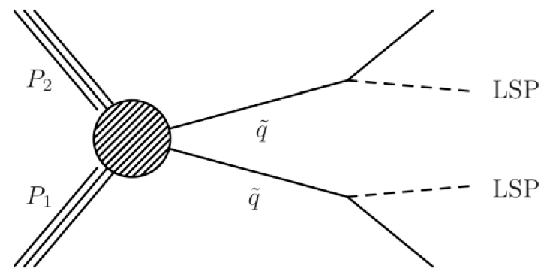
\includegraphics[width=.5\textwidth]{images/pdf/standard_razor_susy}
    \caption{Simple example of a supersymmetric event, with two heavy
    pair-produced SUSY particles, two invisible lightest supersymmetric
particles and two visible SM particles.}
    \label{fig:standard_razor_susy}
\end{figure}
In this kind of events, there is an additional, well-motivated approximation
that can be made. If the mass of the heavy particle is sufficiently large
relative to the collider energy $\sqrt{s}$, the particles will be mostly
produced near the threshold $\sqrt{\hat s} \approx 2M$, where
$\sqrt{\hat s}$ is the usual Mandelstam variable describing the hard
partonic process.
In this approximation, we can move from the laboratory reference frame to
the centre-of-mass frame of the pair-produced particles by finding the frame
where the magnitude of the momenta $\vec a$ and $\vec b$ of the visible particles are equal. This
frame is called the \emph{R frame}.
We define the R-frame mass $M_{R0}$ as:
\begin{equation*}
    M_{R0} \mathop:= \sqrt{(a^0 - b^0)^2 - (a^3 + b^3)^2}
\end{equation*}
Where $a^\mu$ and $b^\mu$ are the four momenta of the visible particles, as
measured in the laboratory frame.
This quantity is invariant under longitudinal boosts, and has a distribution
peaked at the value of the massive particle's mass.

It is not invariant under boosts in the transverse plane, but the
effects of the \pt of the pair-produced particles can be taken into account.
Introducting the notation $\vec{v}_T = (v_x, v_y, 0)$ for the transverse
components of any vector $\vec{v}$, $\vec m$ for the vector representing the
\met, the corrections in~\cite{chris_email}
can be applied:
\begin{align*}
    \vec u \mathop: &= \vec a + \vec b + \vec m\\
    \vec v \mathop: &= \vec a + \vec b\\
    M_R^2 &= \dfrac{1}{2}\left\{ M_{R0}^2  - \vec{u}_T \cdot \vec{v}_T 
    + M_{R0}\sqrt{M_{R0}^2 + \vec{u}_T^2 - 2\vec{u}_T \cdot \vec{v}_T}\right\}
\end{align*}

\section{The transverse plane and the $R$ variable}\label{sec:r}
Traditionally, the requirements used to improve the signal to background
ratio in these processes is large magnitude of the missing transverse
energy.
However, by looking at the formula for $M_R$ in the previous section, we see
that there is additional kinematical information not yet used. That is,
apart from the small correction for the \pt of the massive particle, the
quantities in the transverse plane are not used in the calculation of the
$M_R$ variable.

We then assign half of the measured \met to each escaping particle,
and define:
\begin{equation*}
    M_{R}^T = \sqrt{\dfrac{|\vec{m}|}{2}(|\vec{a}_T| + |\vec{b}_T|) -
    \dfrac{\vec m}{2}\cdot (\vec{a}_T + \vec{b}_T)}
\end{equation*}
This variable is an additional measurement of the scale of the process, that
uses the information independent of the $M_R$. Finally we form the
dimensionless $R$ variable as the ratio:
\begin{equation*}
    R\mathop:= \dfrac{M_R^T}{M_R}
\end{equation*}
For signal processes, the distribution of $R$ peaks near \nicefrac{1}{2}
since it is the ratio of two measurements of the same scale, while for
background events it is expected to fall after reaching a maximum for a
lower value.

The effects of the \pt of the massive particle are taken into account by
using the same formula for $M_R^T$ but by boosting the vectors $\vec a$,
$\vec b$ and $\vec m$ by their sum $\vec a + \vec b + \vec m$.

\section{The razor variables for the top partners}
The top partner event topology is different from the mentioned
supersymmetric example, as the decay chains of the pair-produced particles
are different: one of them decays into two leptons and one b-jet, while the
other one decays into many jets
(figure~\ref{fig:susy_toppartner_comparison}).
\begin{figure}[h]
    \centering
    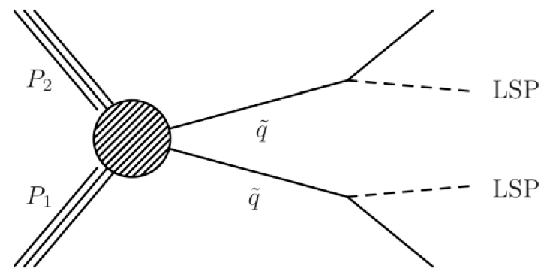
\includegraphics[width=.5\textwidth]{images/pdf/standard_razor_susy}
    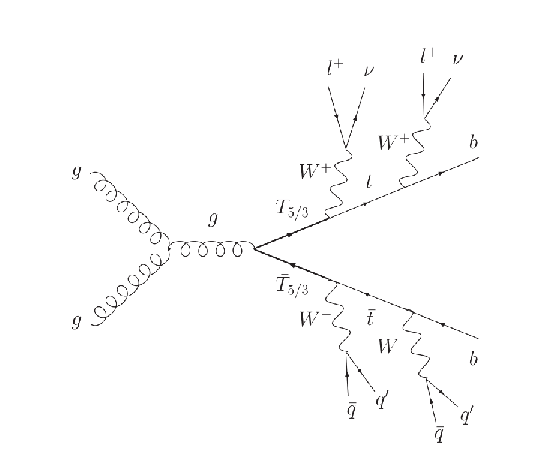
\includegraphics[width=.5\textwidth]{images/pdf/TTbar_feynman}
    \caption{Comparison of a simple supersymmetric example
        with
    the top partner decay.}
    \label{fig:susy_toppartner_comparison}
\end{figure}
The obvious approach would be to try to build two \emph{pseudoparticles} by
summing the four momenta of the decay products of each \TP in the event. This was
done in other SUSY searches for a variety of final
states\cite{CMS-PAS-SUS-11-024}.
However, this does not give good results in \TP events for a number of 
reasons:
\begin{itemize}
    \item there is a combinatorial background given by the fact that
        one of the jets belongs to one particle, and at least four jets to
        the other particle
    \item the \met is no longer equally shared by the two decay branches,
        but should be associated to the branch containing the two leptons
    \item there is high-quality information from the leptons, which are very
        well reconstructed at CMS. These kinematical features get smeared by
        the mixing with the jets, which are more complex and noisier
        objects
\end{itemize}
A new approach was sought for solving these problems, and the solution is at
the same time simple, elegant and powerful.
The idea is to build a \emph{razor subsystem} containing only the two
leptons and the two neutrinos. This follows exactly the basic topology
outlined in~\ref{sec:mr} and~\ref{sec:r} for SUSY events, and the $M_R$
variable is expected to have a peak at half the mass of the \TP.

The jets can then be analyzed as a hadronic system. Since this system is, in
principle, completely reconstructed, we measure its invariant mass.

The hadronic invariant mass and $M_R$ in figures~\ref{fig:had_mass}
and~\ref{fig:mr_nobtag} show that the discriminating power of these
variables is already very good. The prediction that the $M_R$ variable peaks
at half the mass of the \TP is also confirmed. We can also see a
reconstruction of the mass of the \Z boson in double electron events with
charge misidentification, again showing the robustness of this method.
On the contrary, the $R$ variable has a very
broad distribution.

\begin{figure}[htb]
    \centering
    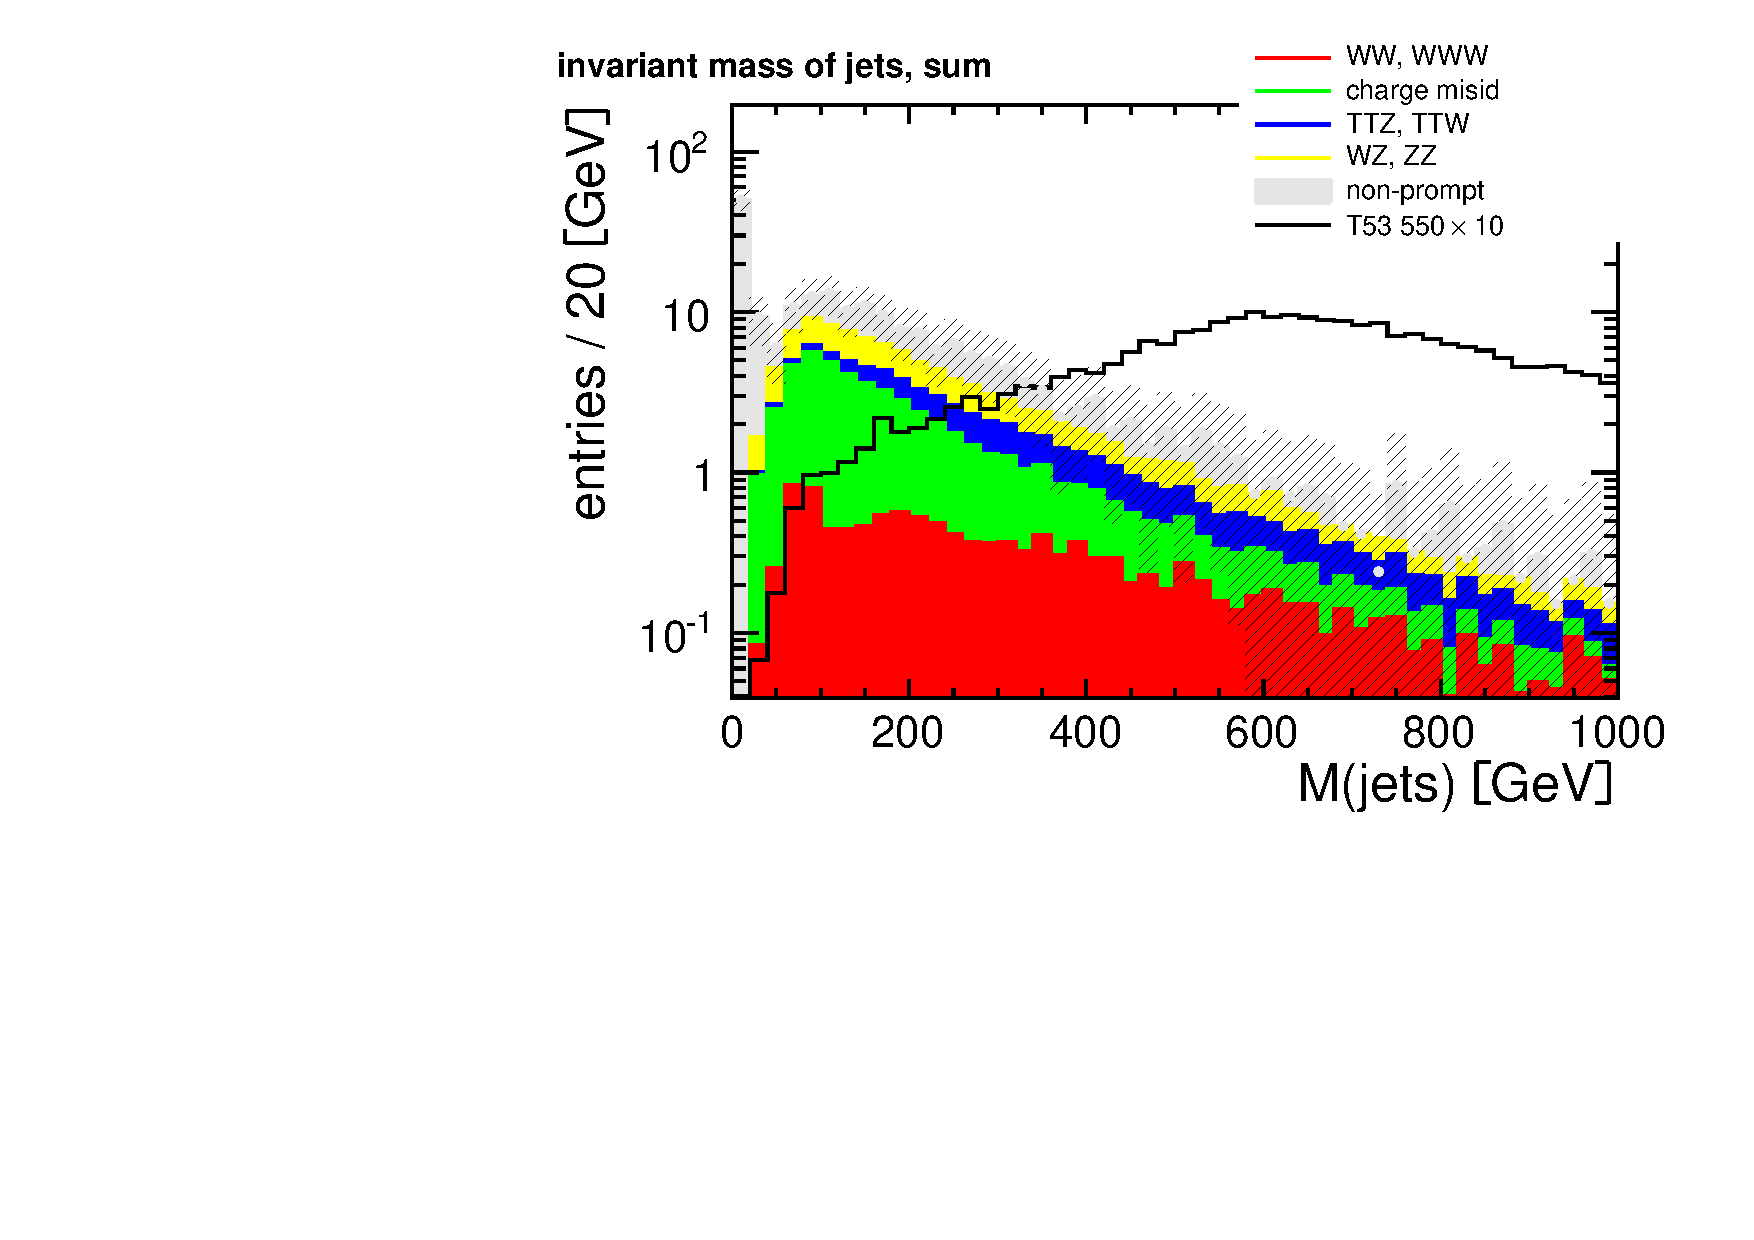
\includegraphics[width=.8\textwidth]{images/pdf/had_mass_sum_0}
    \caption{Invariant mass of the hadronic system for the sum of the three decay channels. Events with two same-sign leptons and at least
two jets are shown. The plots for the \E\E, \E\M, \M\M\ channels are
shown in figure~\ref{fig:had_mass_app}}
    \label{fig:had_mass}
\end{figure}

\begin{figure}[htb]
    \centering
    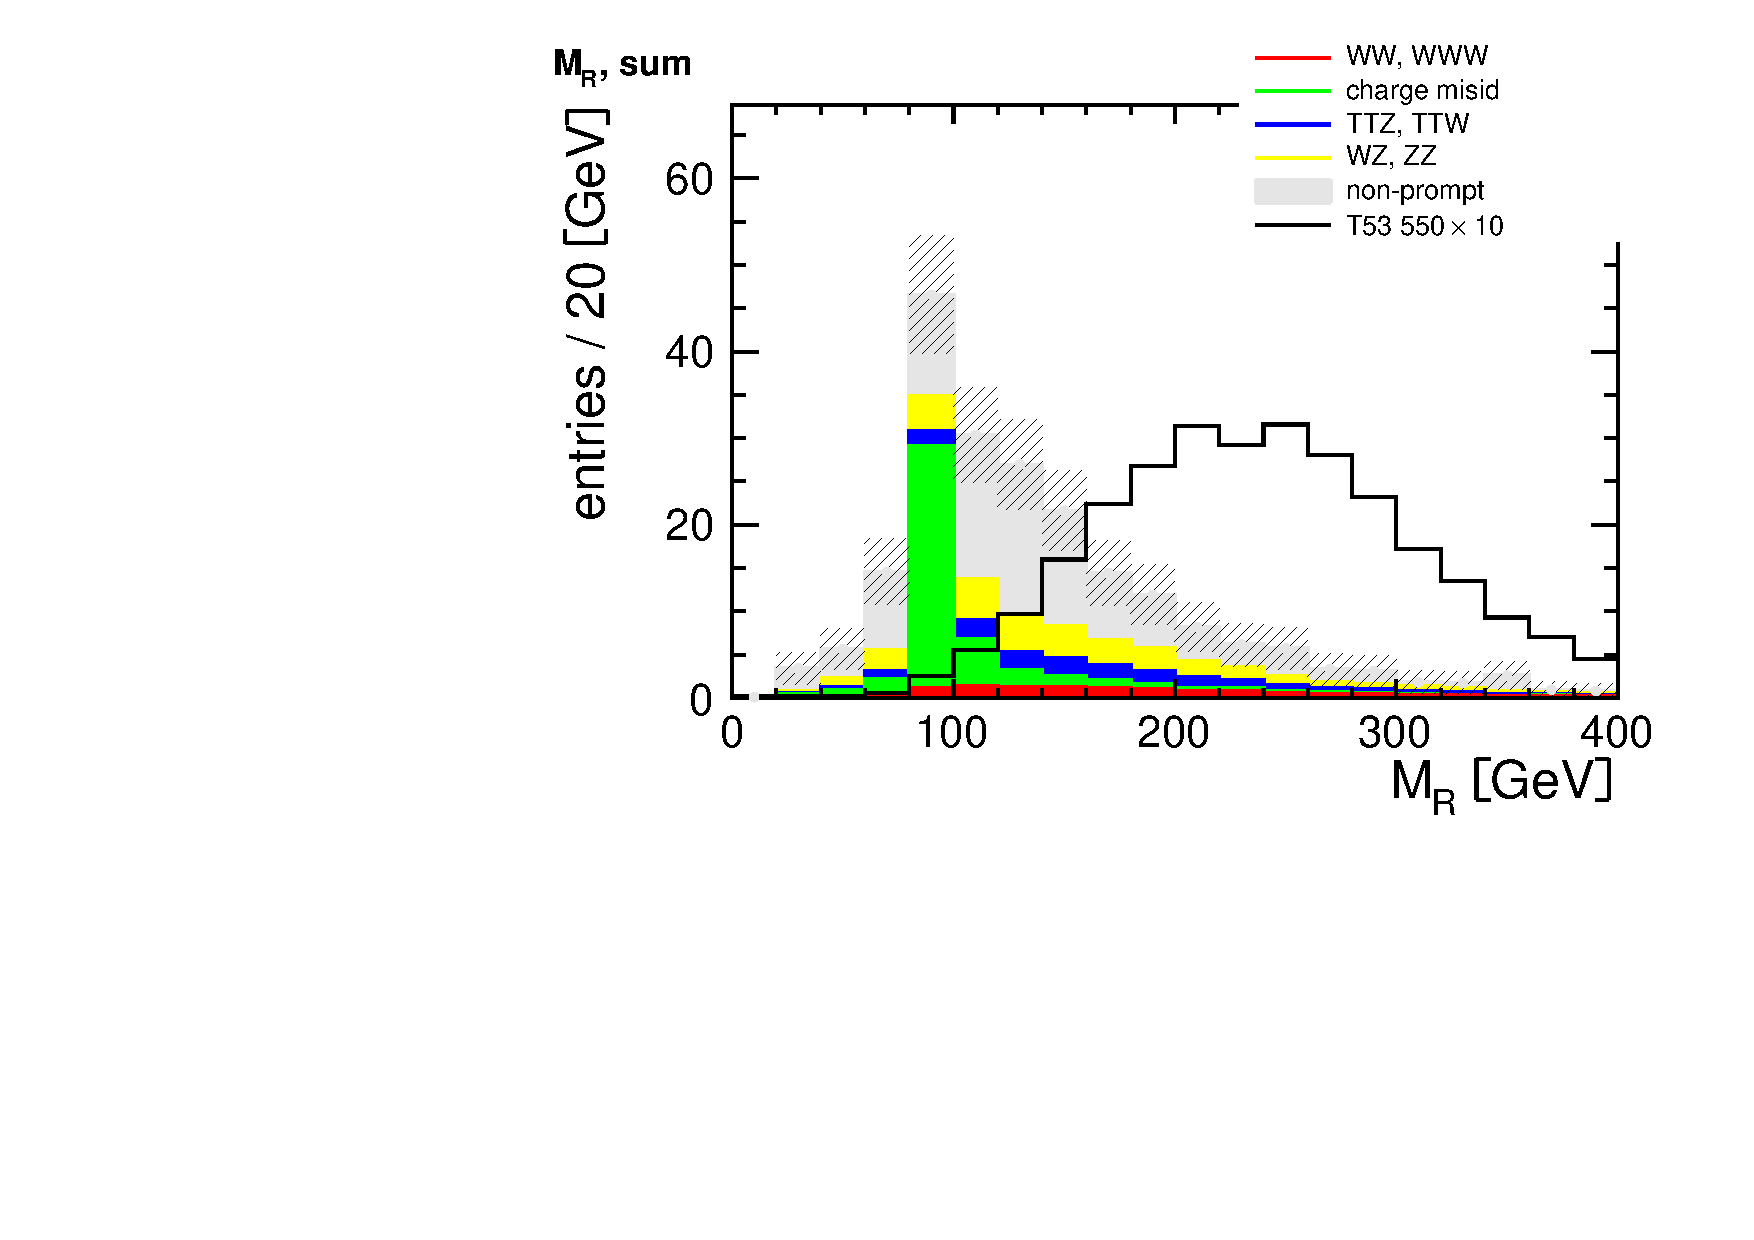
\includegraphics[width=.8\textwidth]{images/pdf/mr_sum_0}
    \caption{$M_R$ distributions for the sum of the three decay channels. Events with two same-sign leptons and at least
two jets are shown. The plots for the \E\E, \E\M, \M\M\ channels are
shown in figure~\ref{fig:mr_nobtag_app}}
    \label{fig:mr_nobtag}
\end{figure}

\begin{figure}[htb]
    \centering
    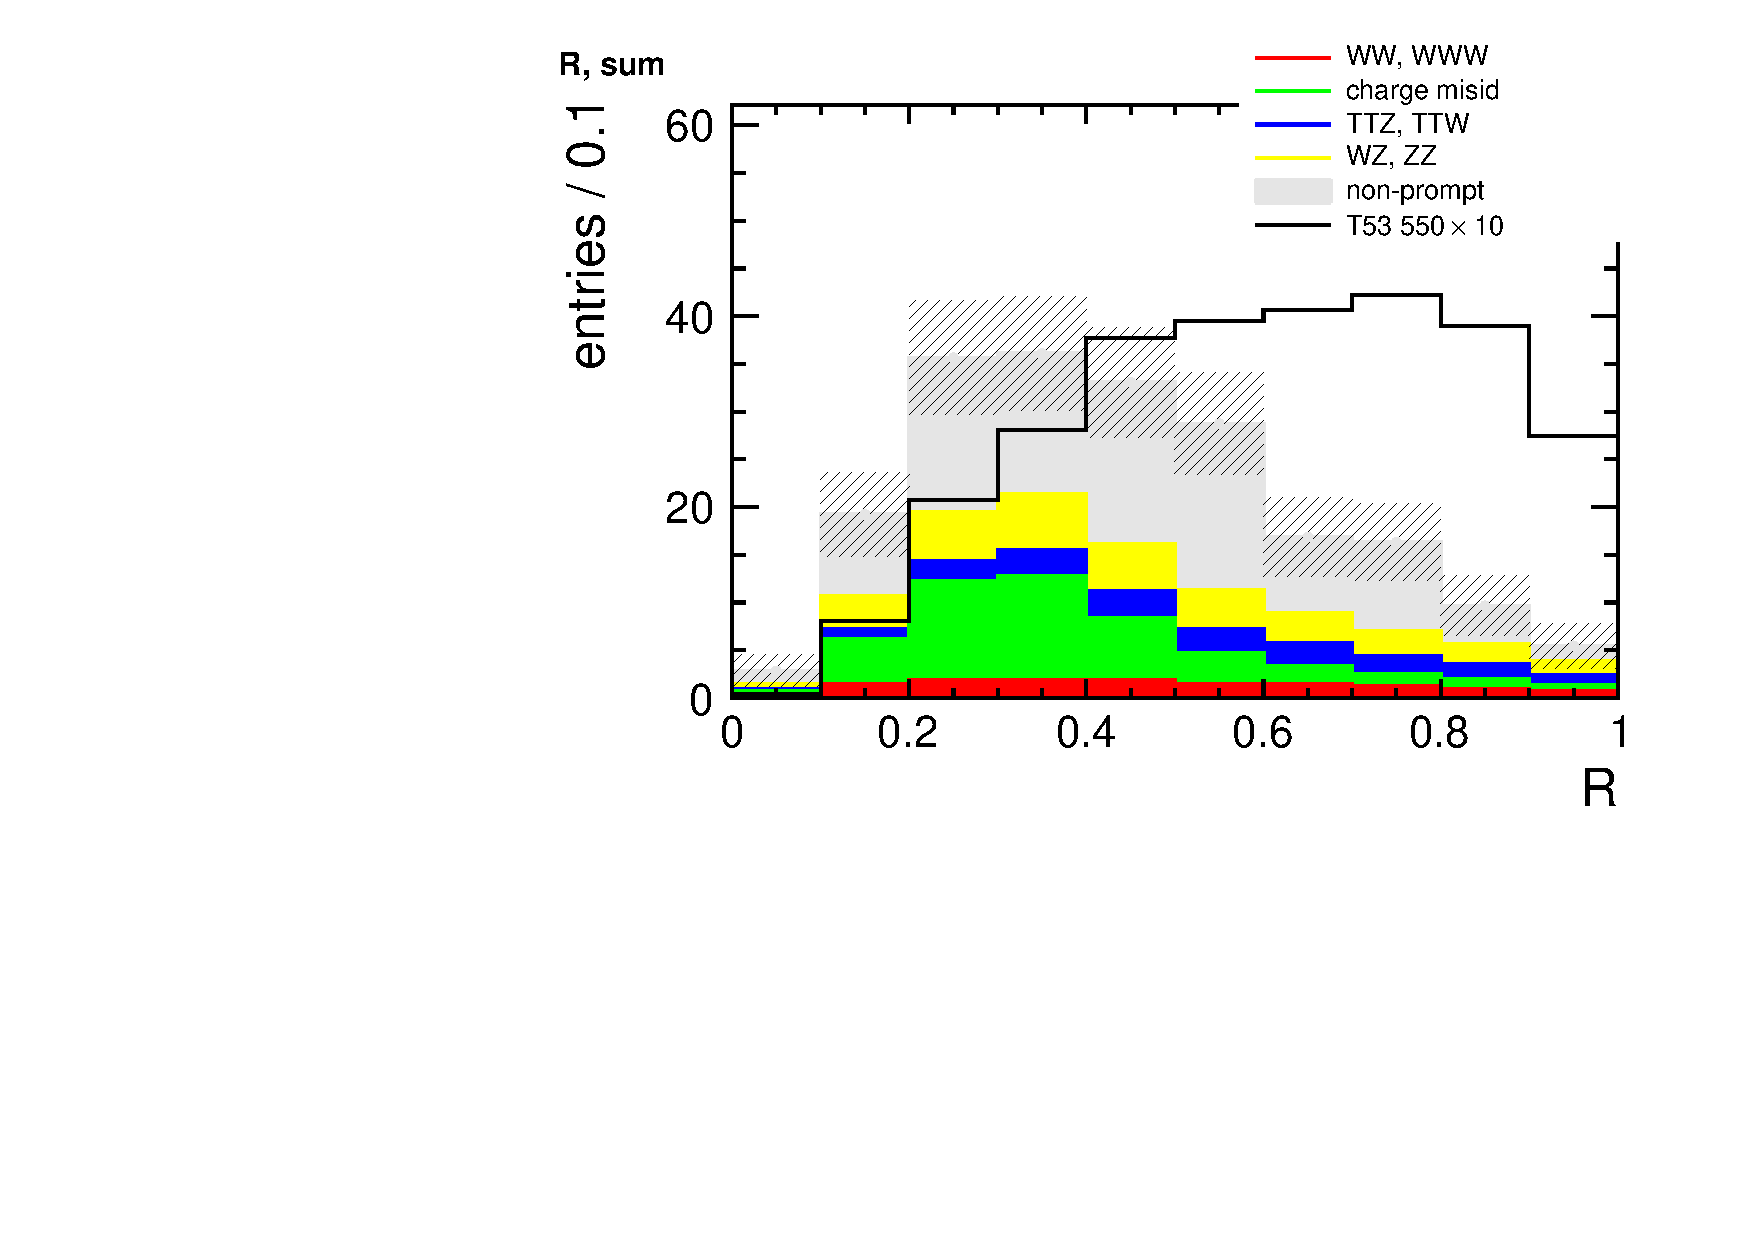
\includegraphics[width=.8\textwidth]{images/pdf/r_sum_0}
    \caption{$R$ distributions for the sum of the three decay channels. Events with two same-sign leptons and at least
two jets are shown. The plots for the \E\E, \E\M, \M\M\ channels are
shown in figure~\ref{fig:r_nobtag_app}}
    \label{fig:r_nobtag}
\end{figure}

\section{Event reconstruction improvement and
b-tagging}\label{sec:razor_btagging}
One more approximation remains, that is the association of the b-jet from the leptonic decay
chain to the hadronic system. We can try to identify this jet and add it to
the leptonic system, where it belongs.
From the Monte Carlo information in the signal, we see that this jet is
usually close to the lepton from the top decay
(figure~\ref{fig:dr_jet_lepton}).
\begin{figure}[h]
    \centering
    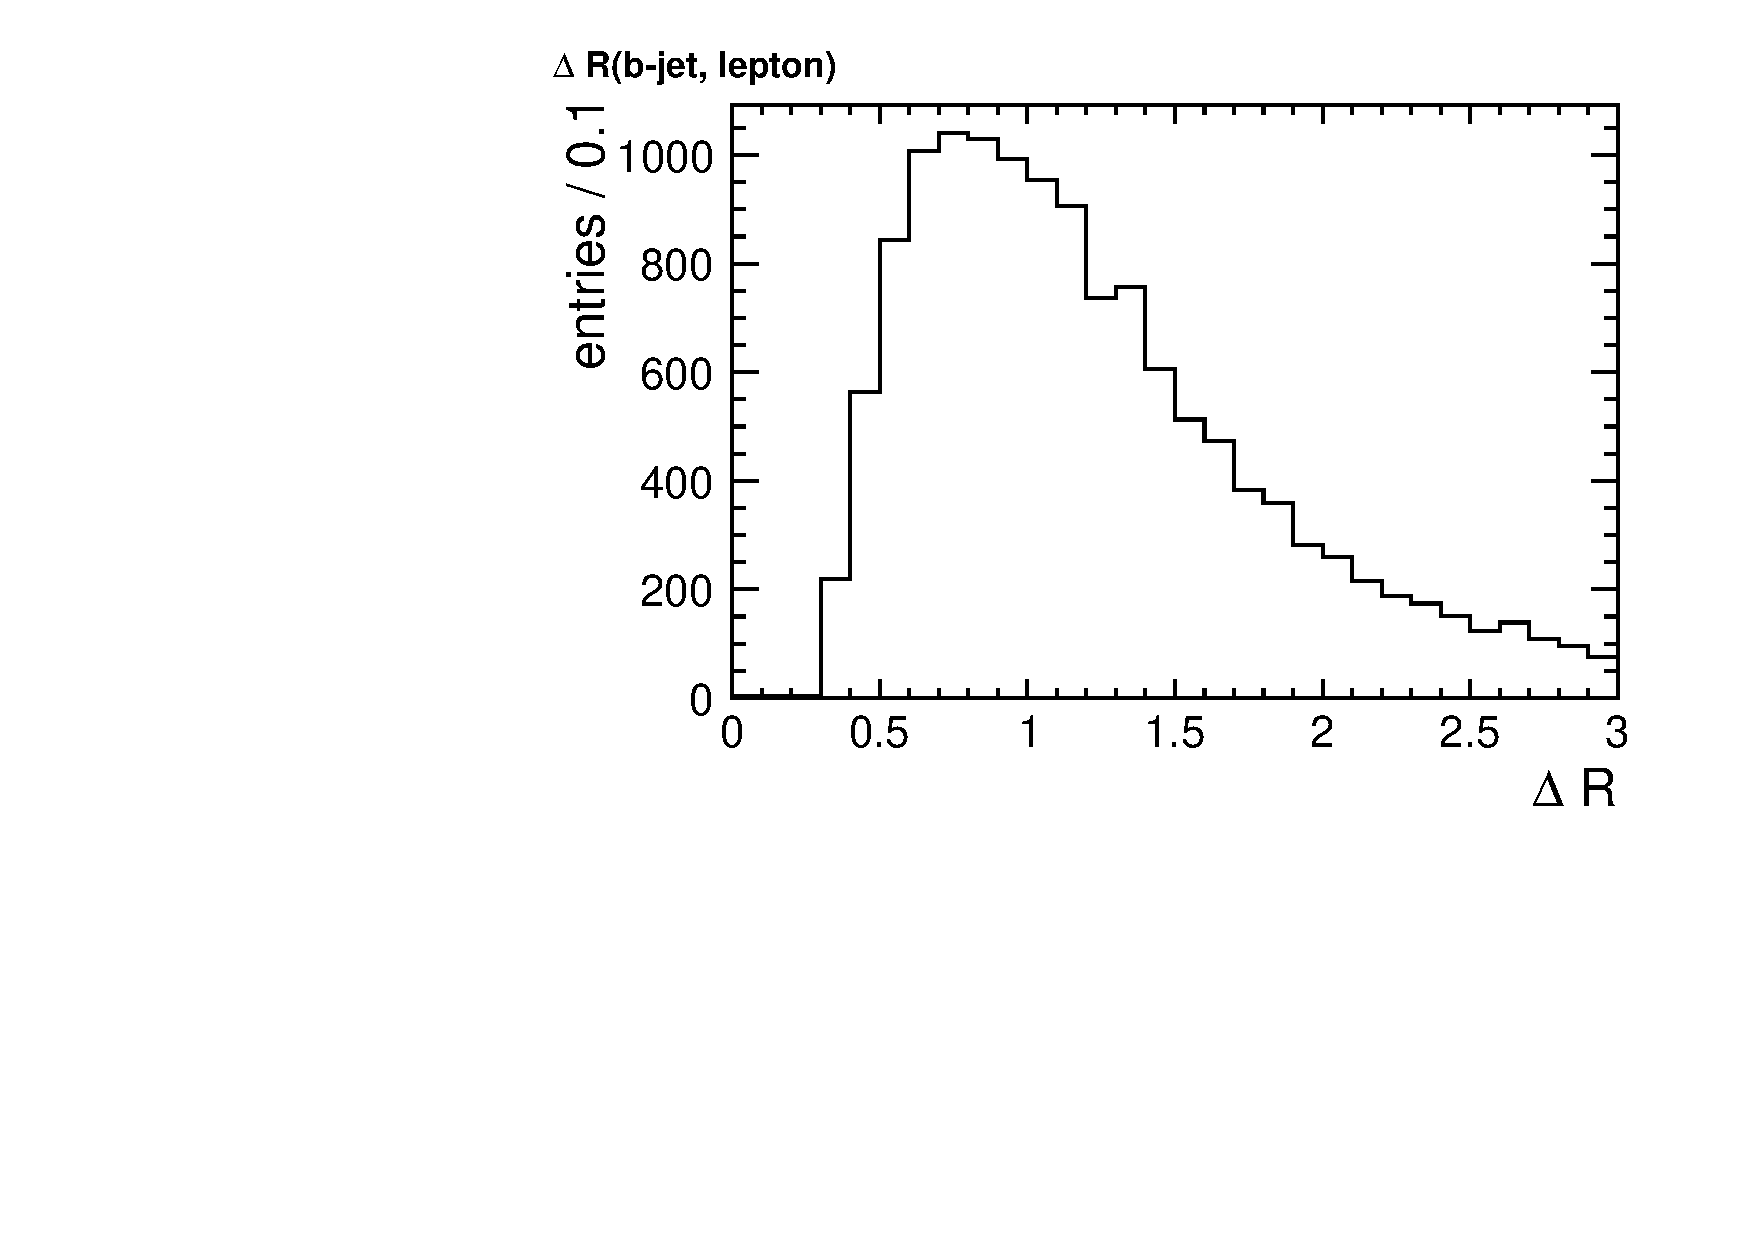
\includegraphics[width=.7\textwidth]{images/pdf/dr_bjet_lepton_canvas}
    \caption{$\Delta R$ between the b-jet and the lepton from the top
        decay. MC truth from the \unit[550]{GeV} mass point.}
        \label{fig:dr_jet_lepton}
\end{figure}
This simple $\Delta R$ matching fails for \nicefrac{2}{3} of the
signal events, mainly because there are two leptons in each event and many
jets. Therefore, an unrelated jet can get close to a lepton just by chance.
Moreover, the b-jet is sometimes not reconstructed because it fails to reach the \pt
threshold (figure~\ref{fig:b_pt}) or it is too close to the lepton itself,
thus failing the $\Delta R < 0.3$ selection of
paragraph~\ref{sec:jet_selection}.


\begin{figure}[h]
    \centering
    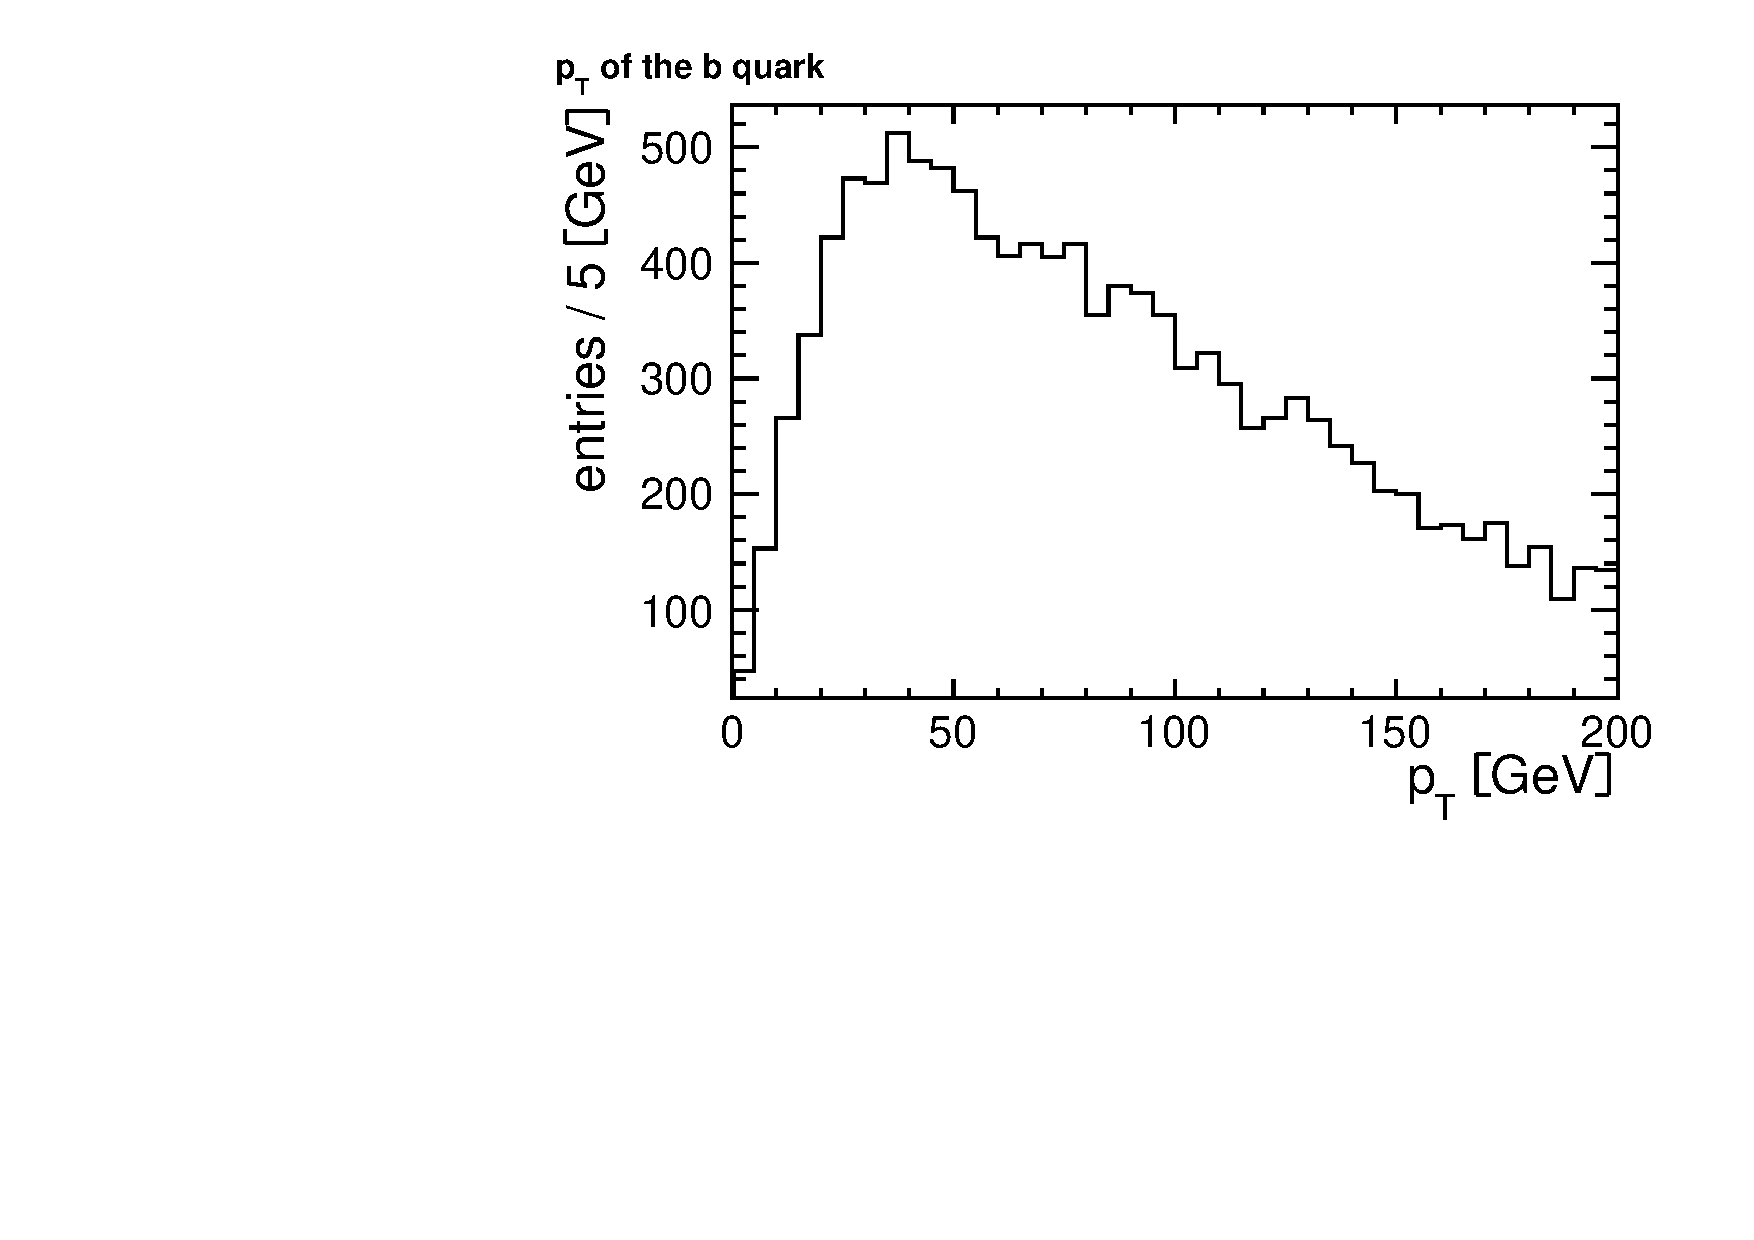
\includegraphics[width=.7\textwidth]{images/pdf/b_quark_pt_canvas}
    \caption{Distribution of the \pt of the $b$ quark in the \TP decay
        chain. If the quark has a low \pt, it will most likely form a
        low-\pt jet, which would not be collected by our selections. MC truth from the \unit[550]{GeV} mass point.}
        \label{fig:b_pt}
\end{figure}

The event reconstruction can indeed be improved with the use of the jet
b-tagging algorithm described in~\ref{sec:btagging}. If two b-tagged jets
are found in the event, the one with the minimum $\Delta R$ with respect to
one of the leptons is moved from the hadronic system to the leptonic system.
The hadronic invariant mass and the razor variables are recalculated
accordingly by summing the four momentum of the b-jet to the leptons, and
subtracting it from the hadronic system at the same time.
If less than two b-tagged jets are found, no association is made.
The studies on the signal show that this improves the event reconstruction
for one in two events. The distributions of the invariant mass and the razor
variables also show an improvement in the background rejection
(figures~\ref{fig:had_mass_optional_btag}, \ref{fig:mr_optional_btag}
and~\ref{fig:r_optional_btag}).

\begin{figure}[htb]
    \centering
    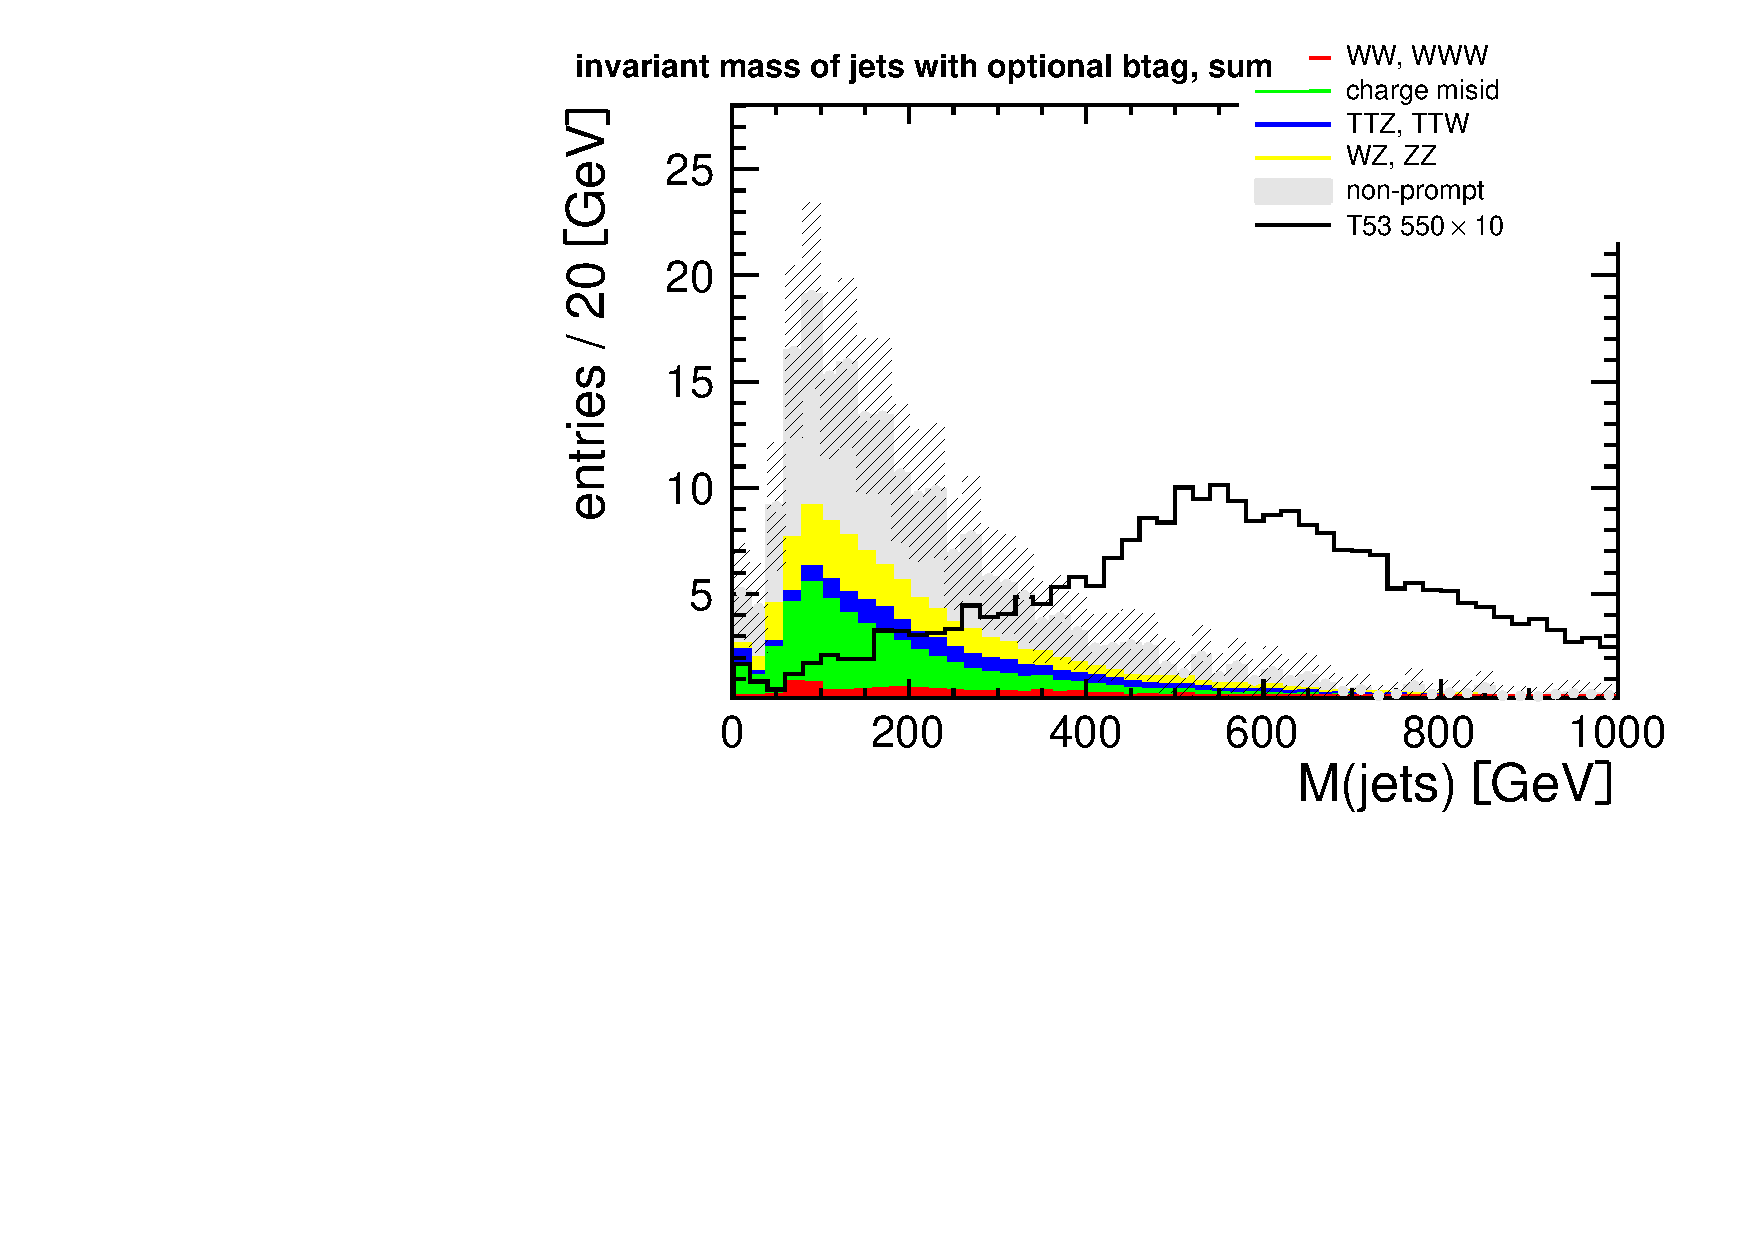
\includegraphics[width=.8\textwidth]{images/pdf/had_mass_optional_btag_sum_0}
    \caption{Invariant mass of the hadronic system for the sum of the three decay channels, with the b-tag correction. Events with two same-sign leptons and at least
two jets are shown. The plots for the \E\E, \E\M, \M\M\ channels are
shown in figure~\ref{fig:had_mass_optional_btag_app}}
    \label{fig:had_mass_optional_btag}
\end{figure}

\begin{figure}[htb]
    \centering
    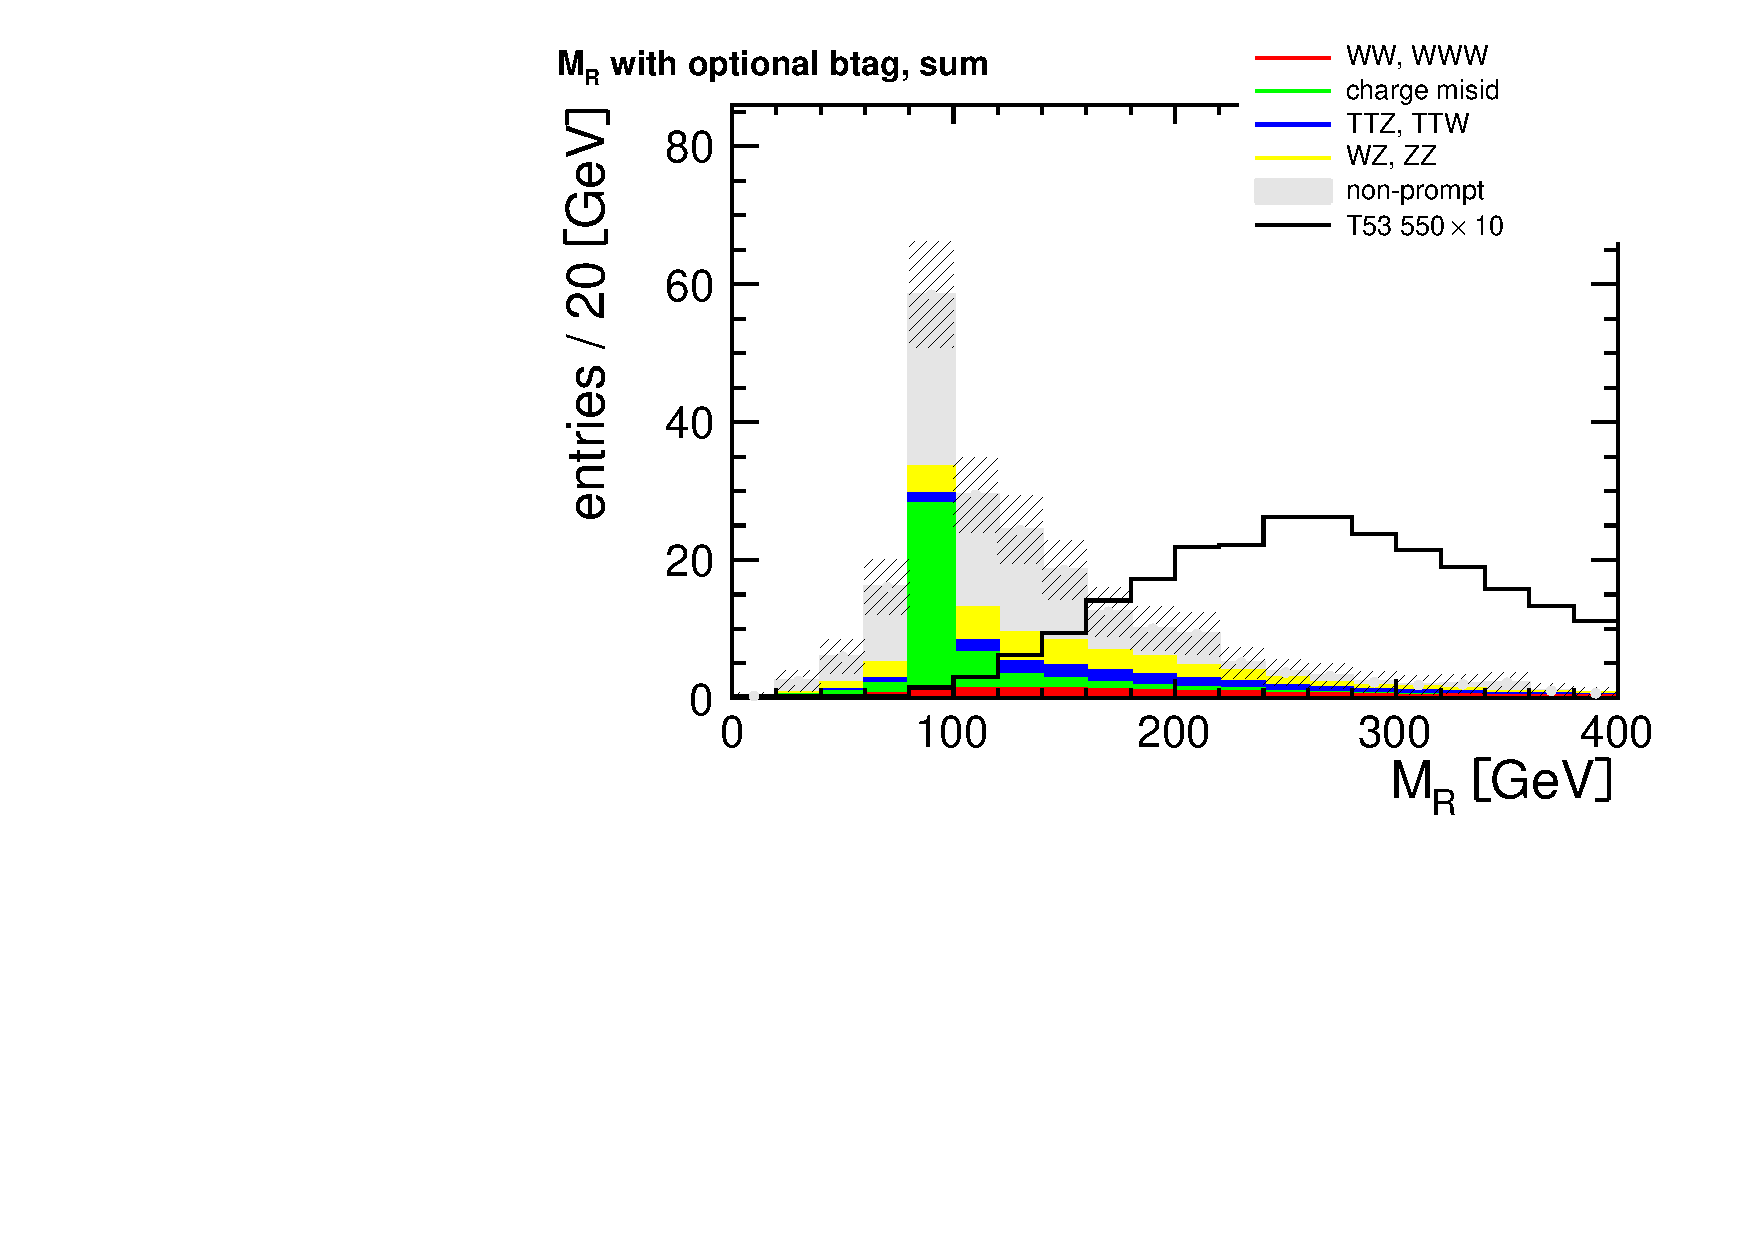
\includegraphics[width=.8\textwidth]{images/pdf/mr_optional_btag_sum_0}
    \caption{$M_R$ distributions for the sum of the three decay channels,
        with the b-tag correction. Events with two same-sign leptons and at least
two jets are shown. The plots for the \E\E, \E\M, \M\M\ channels are
shown in figure~\ref{fig:mr_optional_btag_app}}
    \label{fig:mr_optional_btag}
\end{figure}

\begin{figure}[htb]
    \centering
    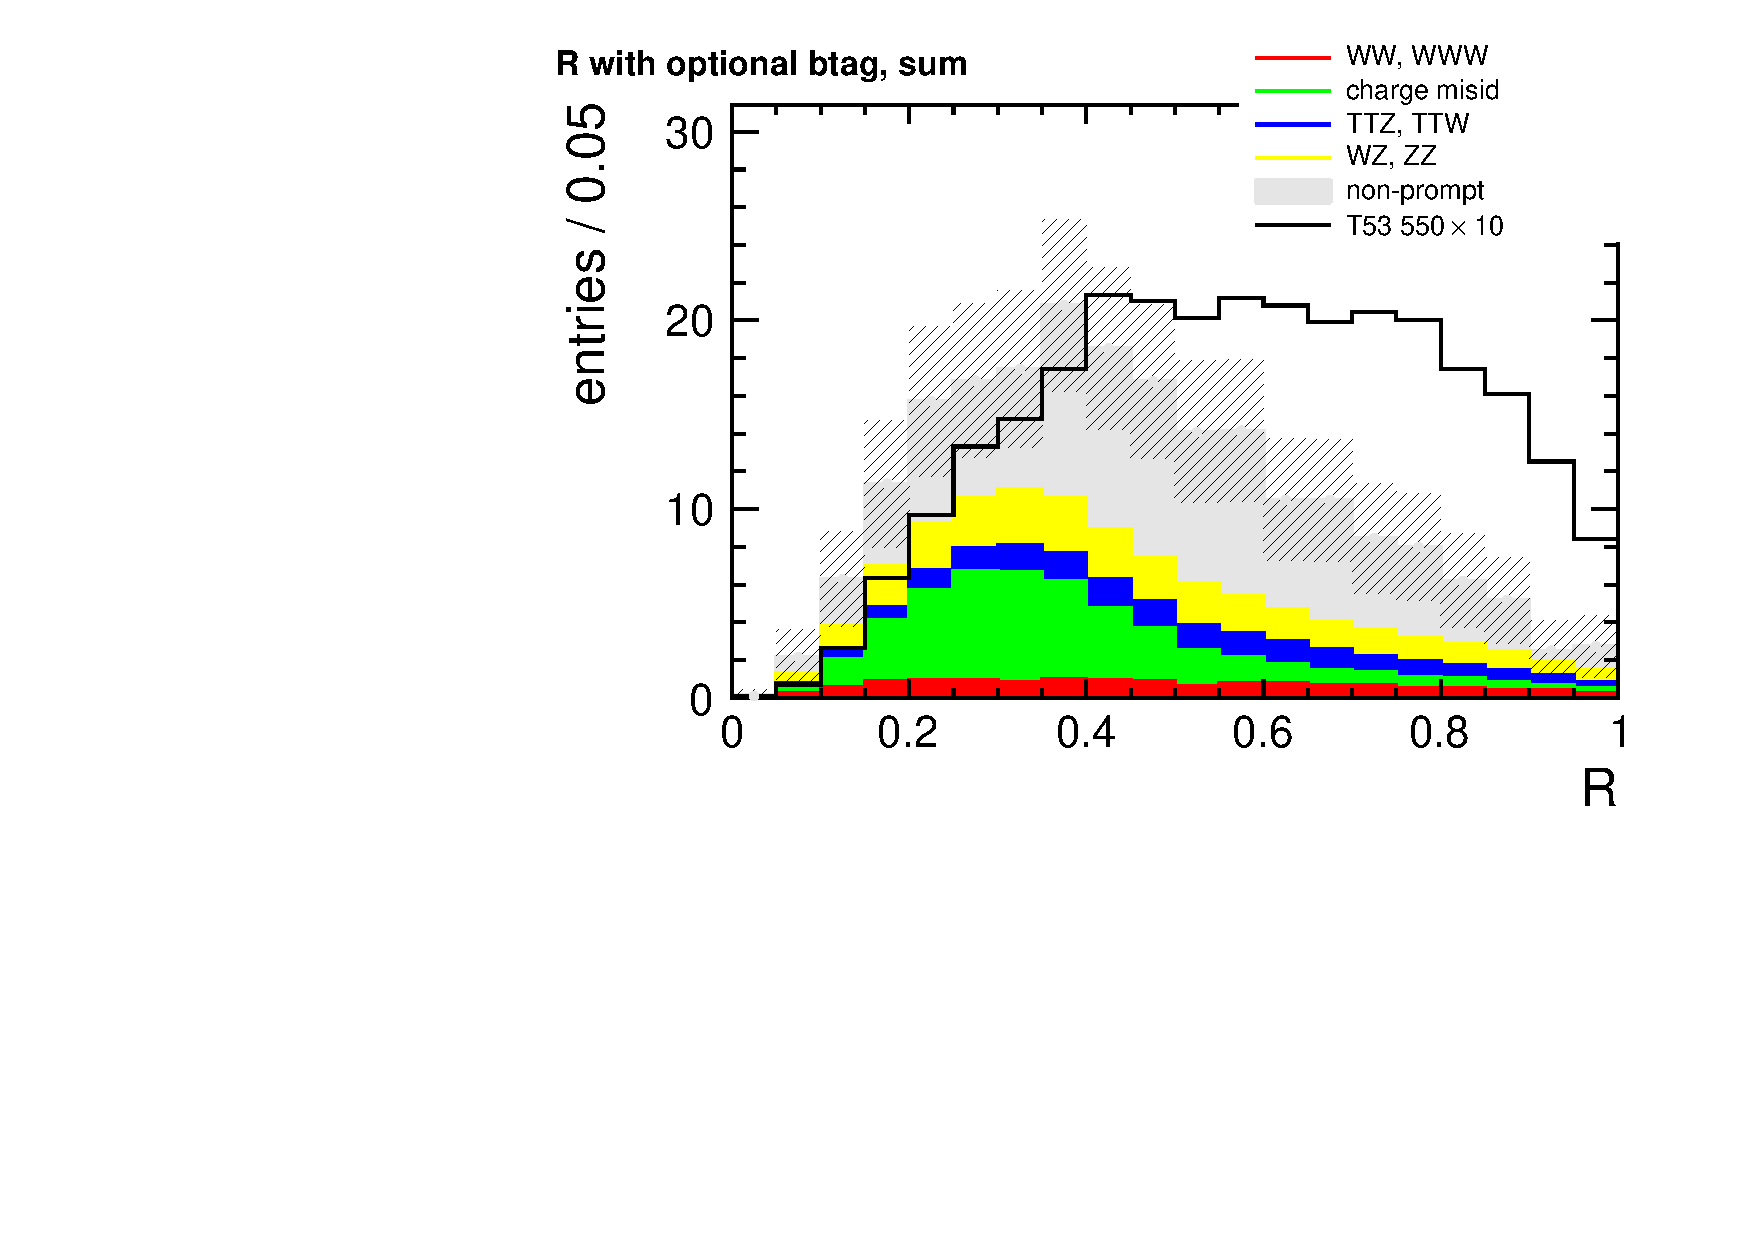
\includegraphics[width=.8\textwidth]{images/pdf/r_optional_btag_sum_0}
    \caption{$R$ distributions for the sum of the three decay channels,
        with the b-tag correction. Events with two same-sign leptons and at least
two jets are shown. The plots for the \E\E, \E\M, \M\M\ channels are
shown in figure~\ref{fig:r_optional_btag_app}}
    \label{fig:r_optional_btag}
\end{figure}

\section{Final event selection}
The razor variables of the last section have to be added to the preselection
described in~\ref{chap:preselection}. There are three variables that can be
used to select candidate \TP events: the invariant mass of the jets, the
$M_R$ and $R$ razor variables. The following selections were chosen to
optimize the ratio\cite{punzi}:
\begin{equation*}
    F \mathop: = \dfrac{\varepsilon(t)}{a/2 + \sqrt{B(t)}}
\end{equation*}
Where $\varepsilon$ is the efficiency of the selection $t$ for the signal,
$B$ is the number of expected background events, and $a$ is the number of
sigmas corresponding to a one-sided gaussian test at significance $\alpha =
95\%$.
The commonly used $S/\sqrt{B}$ figure is unsuitable for the present search,
with a very low background, as the expression breaks down for $B\rightarrow
0$. The ratio $F$ is plotted in figures~\ref{fig:opt_had_mass},
\ref{fig:opt_mr} and~\ref{fig:opt_r}.

\begin{figure}[phtb]
    \centering
    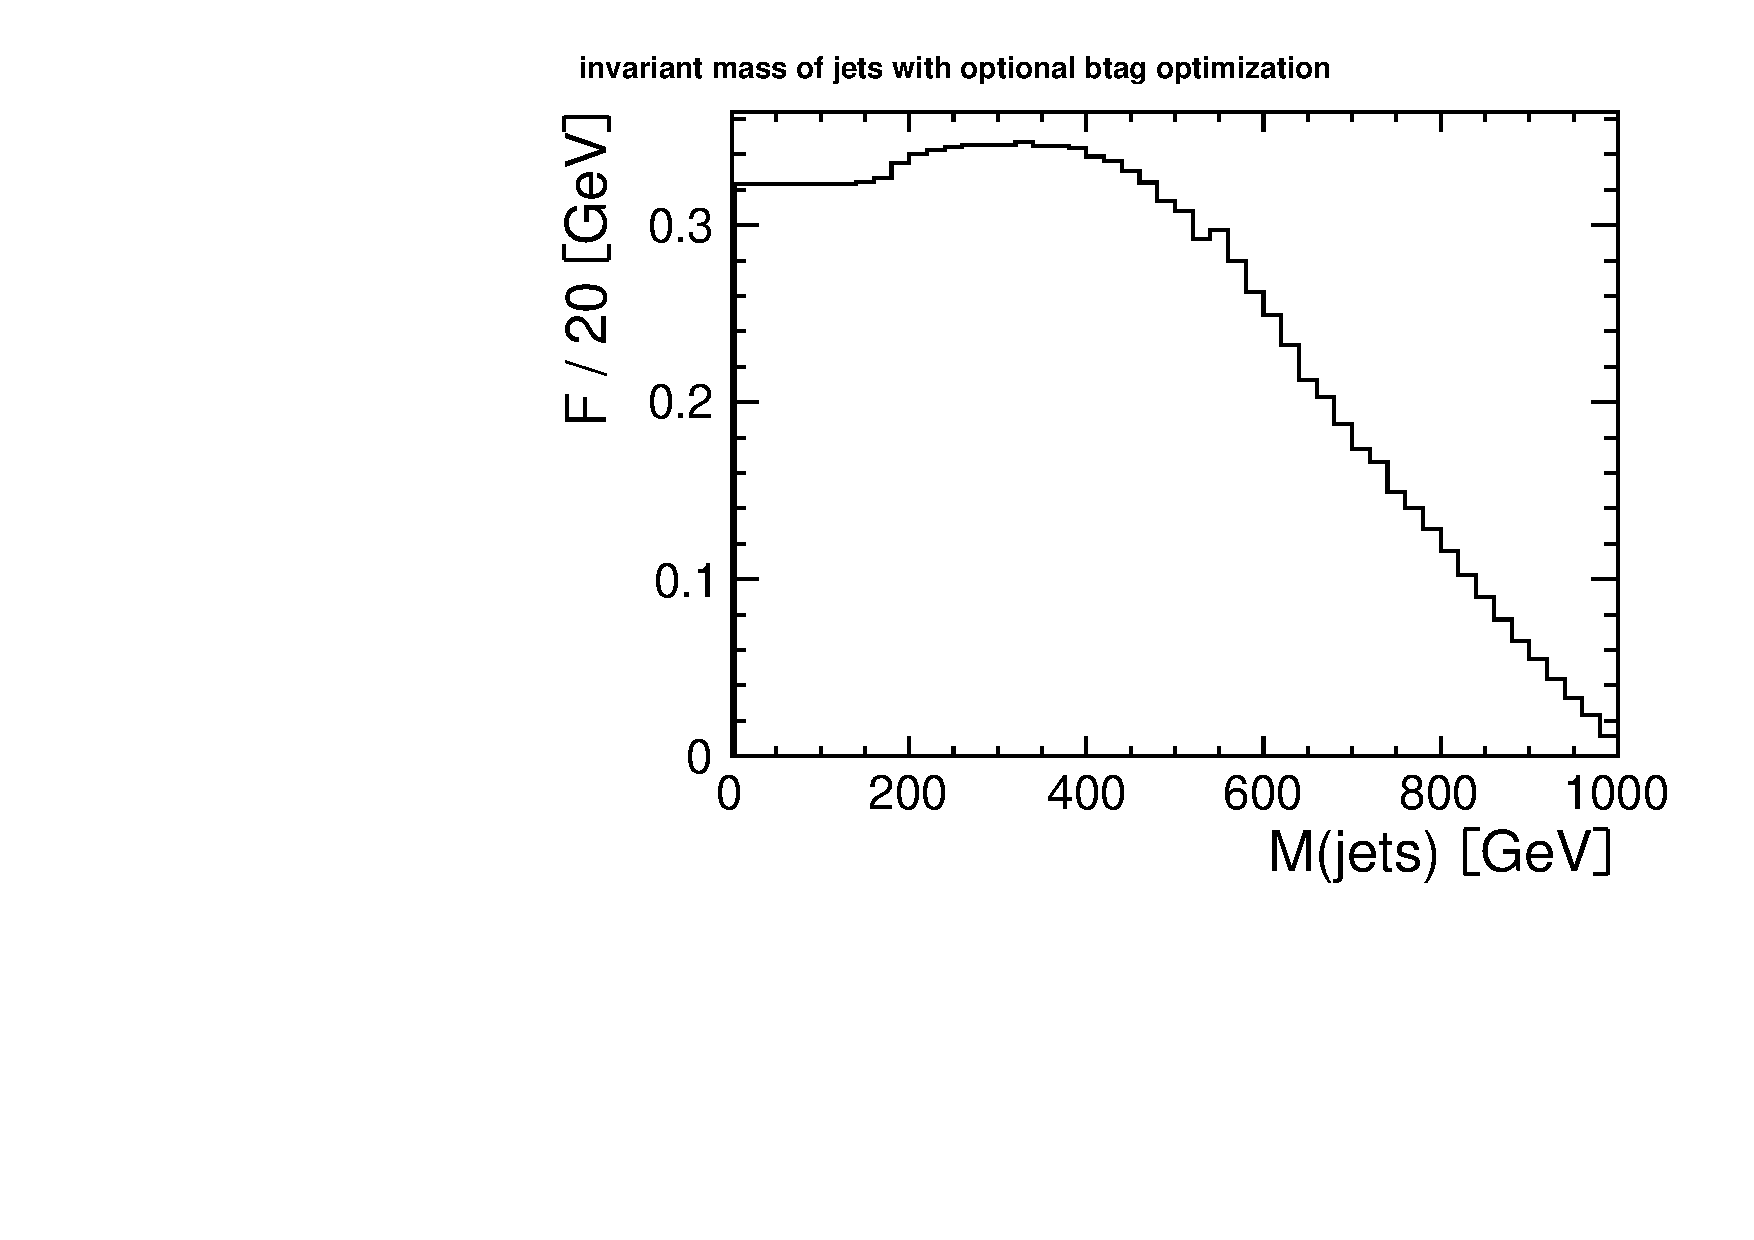
\includegraphics[width=.8\textwidth]{images/pdf/cut_opt_had_mass_optional_btag_4jets_AND_mr200_AND_r02}
    \caption{Optimization figure $F$ for the invariant mass of the hadronic
        system. The selection on $M_R > \unit[200]{GeV}$ and $R > 0.2$ are
    applied. The point where $F$ reaches a maximum is chosen as a cut on this variable.}
    \label{fig:opt_had_mass}
\end{figure}
\begin{figure}[phtb]
    \centering
    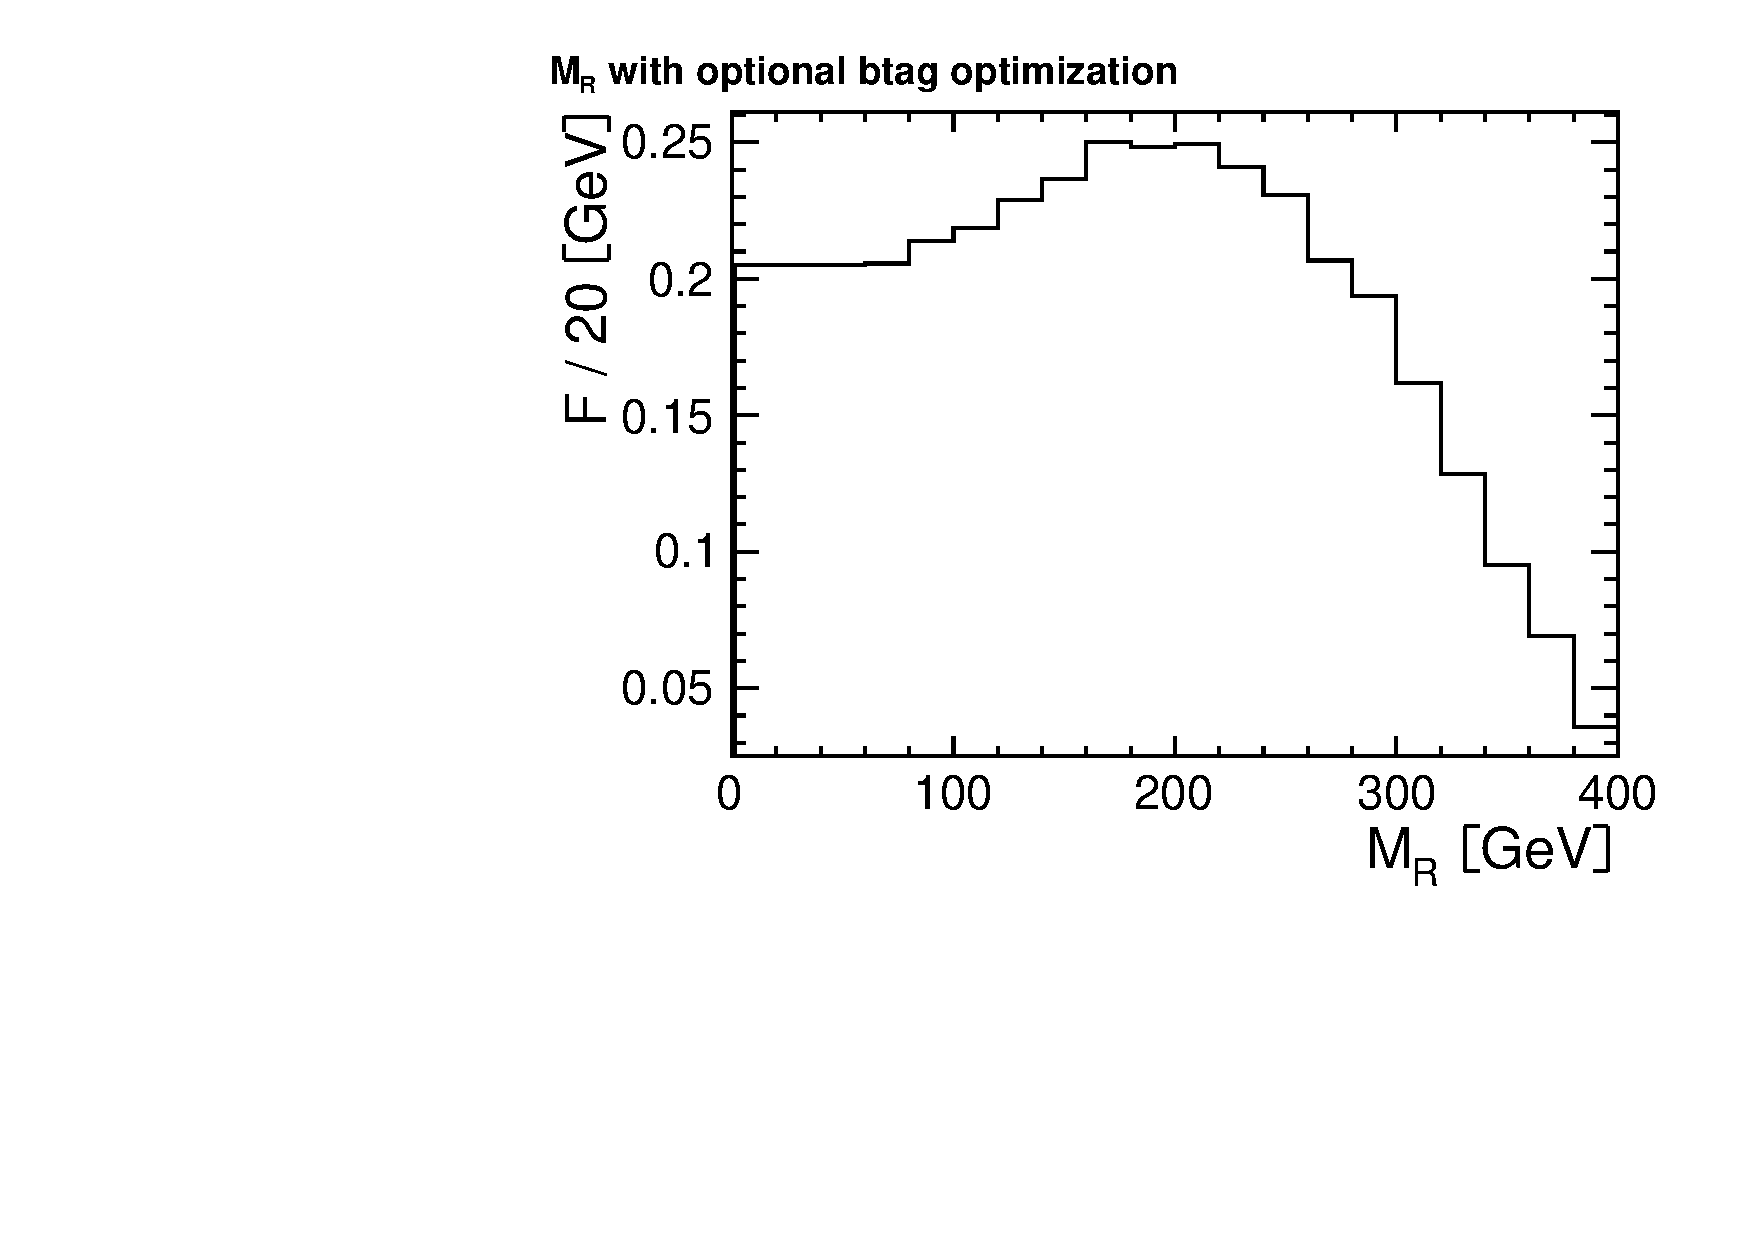
\includegraphics[width=.8\textwidth]{images/pdf/cut_opt_mr_optional_btag_4jets_AND_r02_AND_had_mass350}
    \caption{Optimization figure $F$ for the $M_R$ variable. The selection
        on $M > \unit[350]{GeV}$ and $R > 0.2$ are
    applied. The point where $F$ reaches a maximum is chosen as a cut on this variable.}
    \label{fig:opt_mr}
\end{figure}
\begin{figure}[phtb]
    \centering
    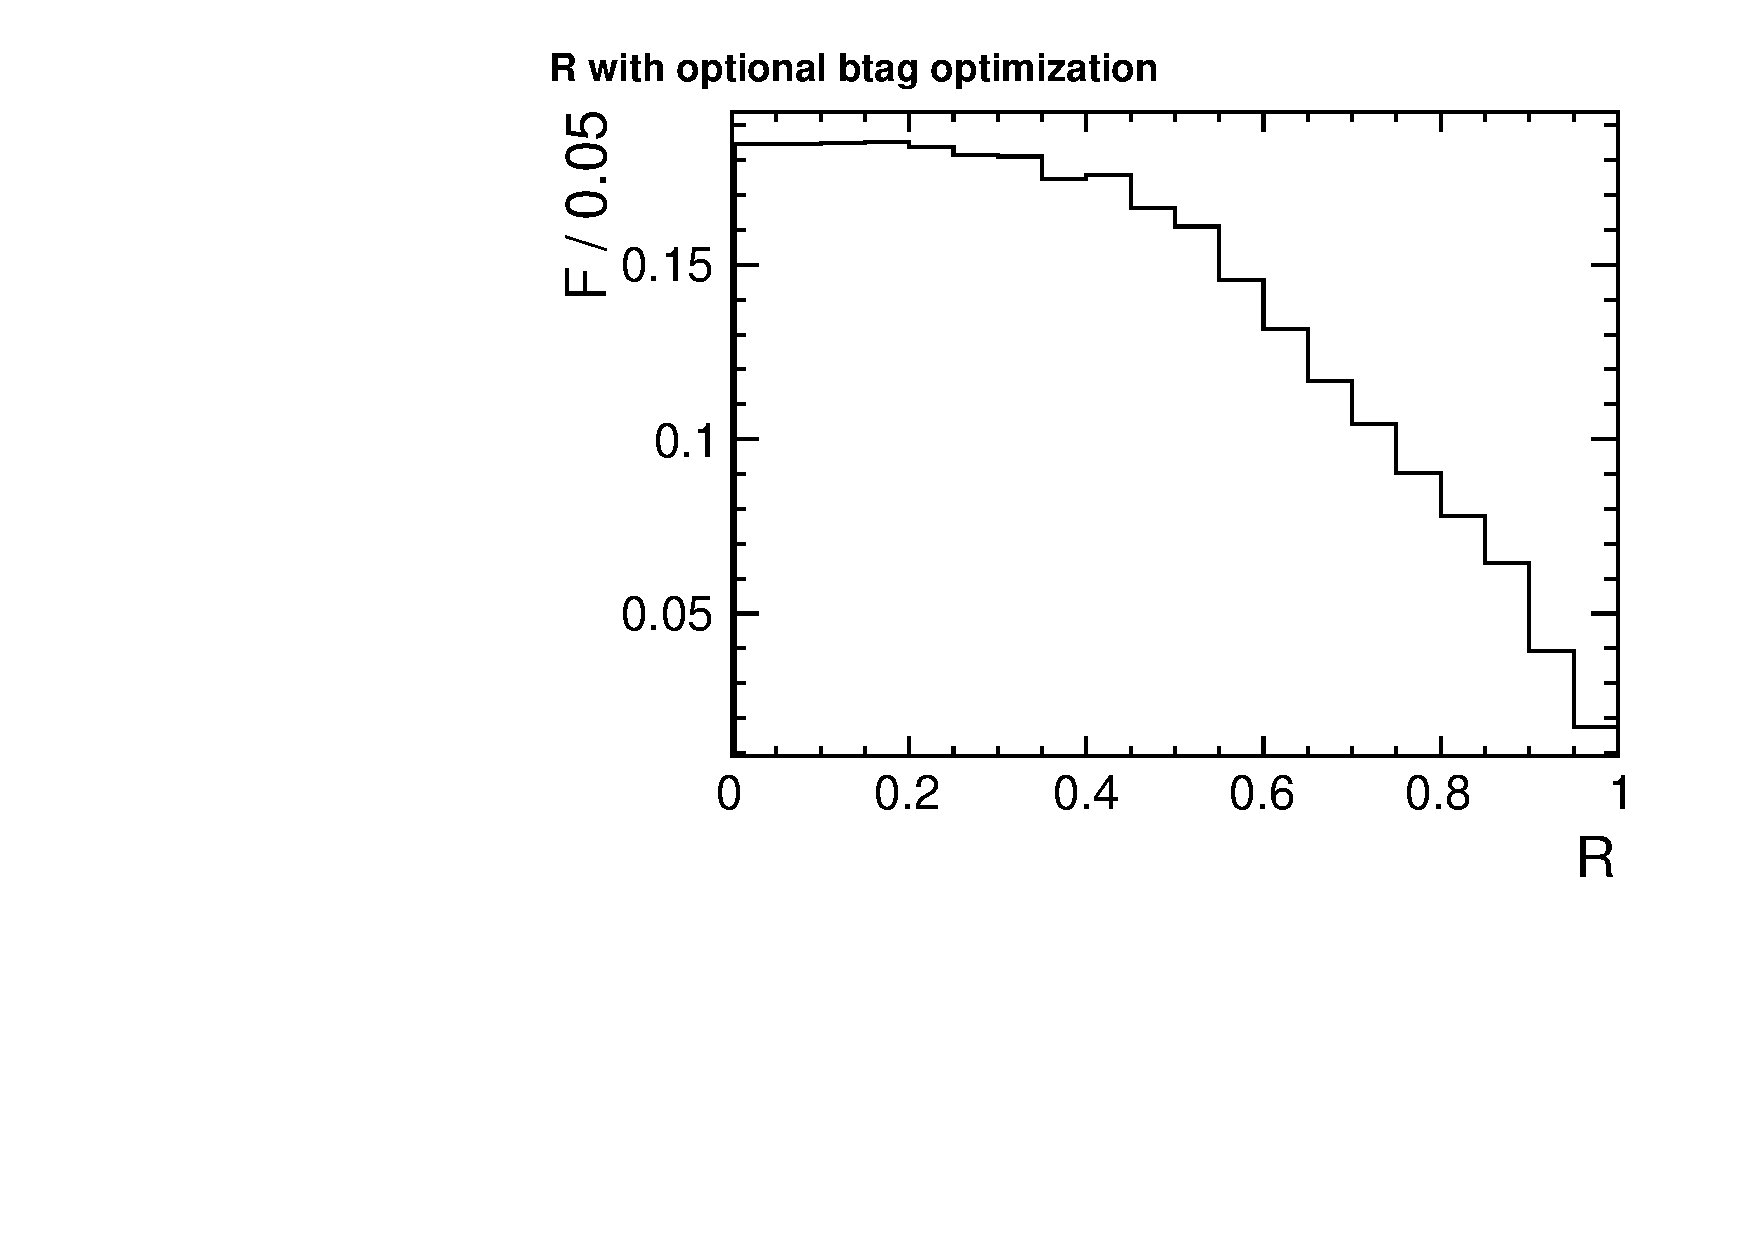
\includegraphics[width=.8\textwidth]{images/pdf/cut_opt_r_optional_btag_4jets_AND_mr200_AND_had_mass350}
    \caption{Optimization figure $F$ for the $R$ variable. The selection
        on $M > \unit[350]{GeV}$ and $M_R > \unit[200]{GeV}$ are
    applied. The point where $F$ reaches a maximum is chosen as a cut on this variable.}
    \label{fig:opt_r}
\end{figure}

The final event selection includes:
\begin{itemize}\label{page:razor_selection}
    \item the event preselection from~\ref{chap:preselection}, with at least
        four jets and invariant mass of the leptons not in the quarkonia and
        \Z boson windows.
    \item invariant mass of the hadronic system greater than
        \unit[350]{GeV}
    \item razor $M_R > \unit[200]{GeV}$
    \item razor $R > 0.2$
\end{itemize}
Figures~\ref{fig:nomr}, \ref{fig:nohadmass} and \ref{fig:nor} show the distributions of the invariant mass of the jets,
$M_R$ and $R$ with all the cuts applied, but the one on the plotted
variable.

\begin{figure}[htb]
    \centering
    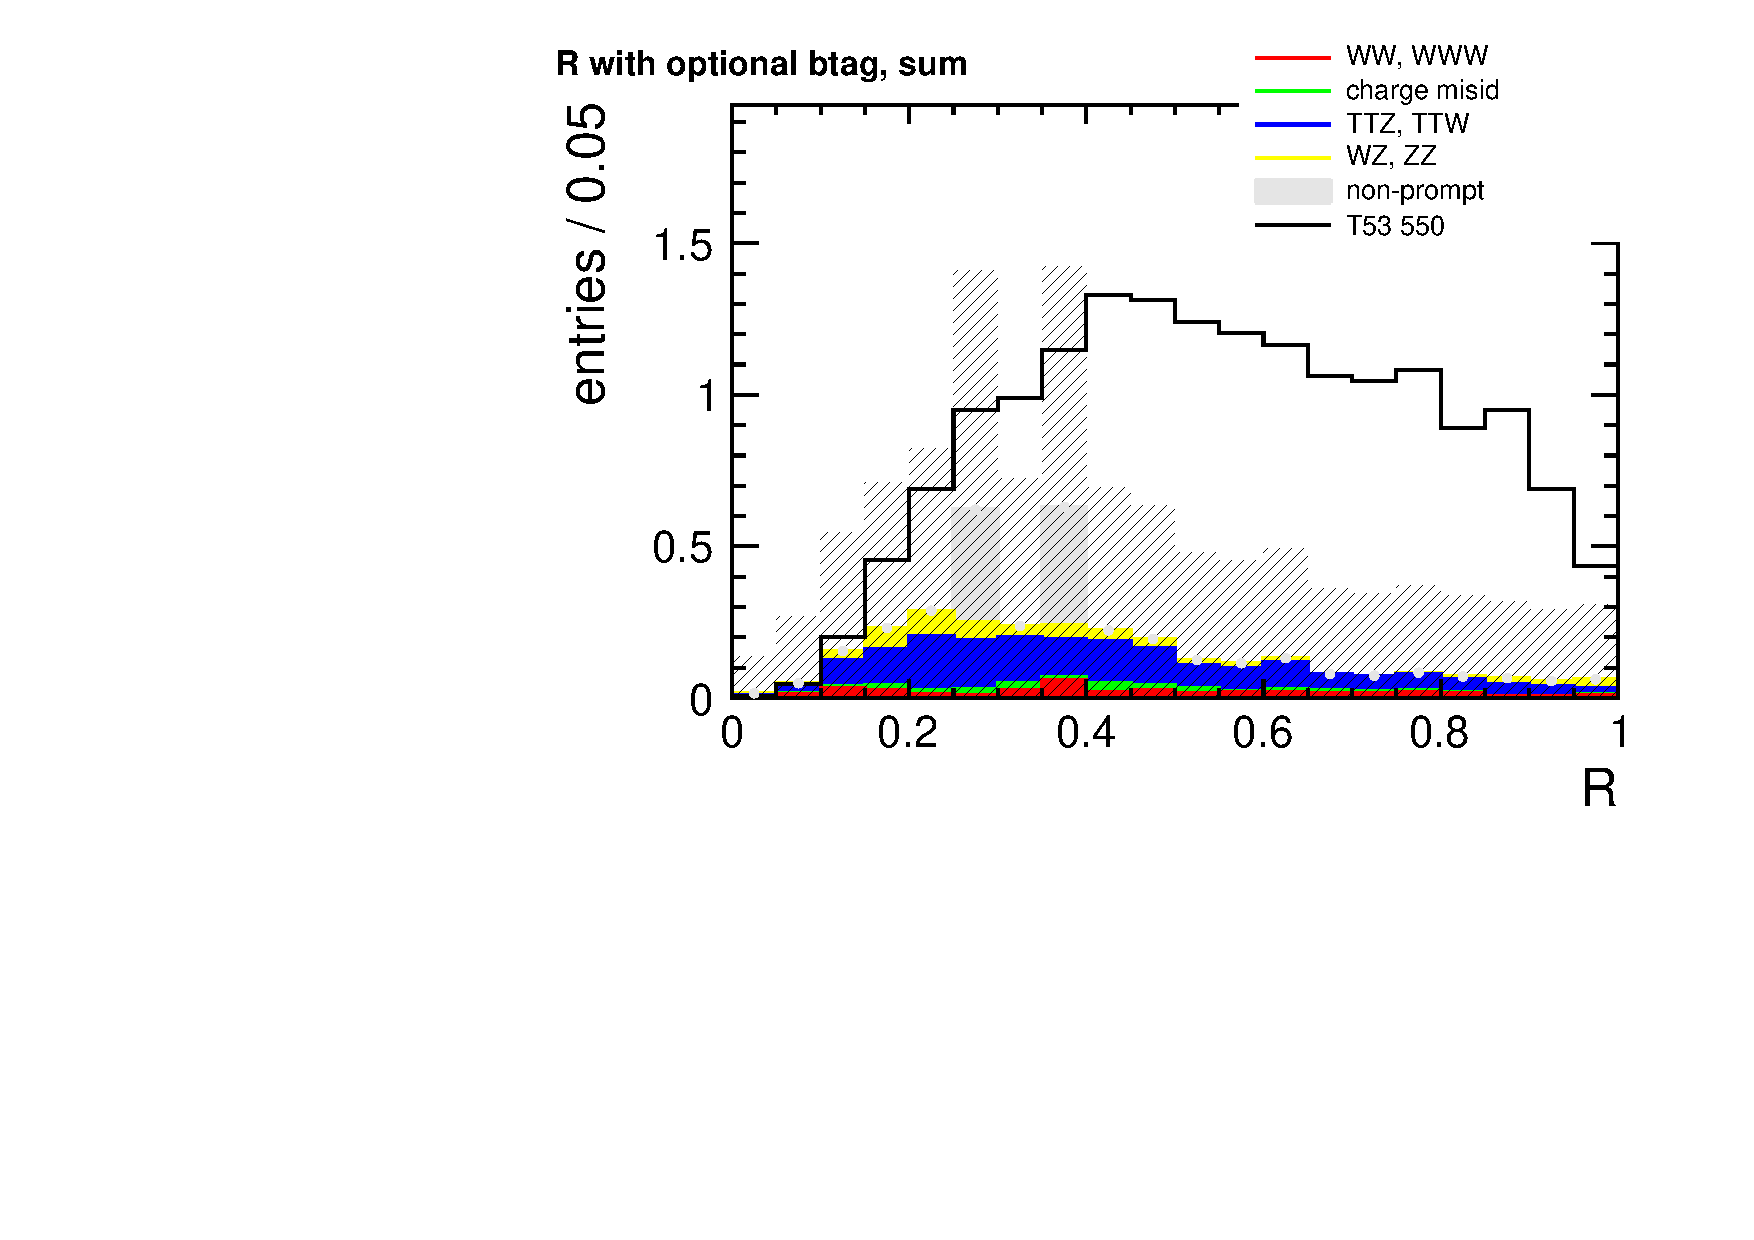
\includegraphics[width=.8\textwidth]{images/pdf/4jets_AND_mr200_AND_had_mass350/r_optional_btag_sum_0}
    \caption{Distribution of the $R$ variable for events in the three decay
        channels, with the final
    selection applied without the selection on $R$.}
    \label{fig:nor}
\end{figure}

\begin{figure}[htb]
    \centering
    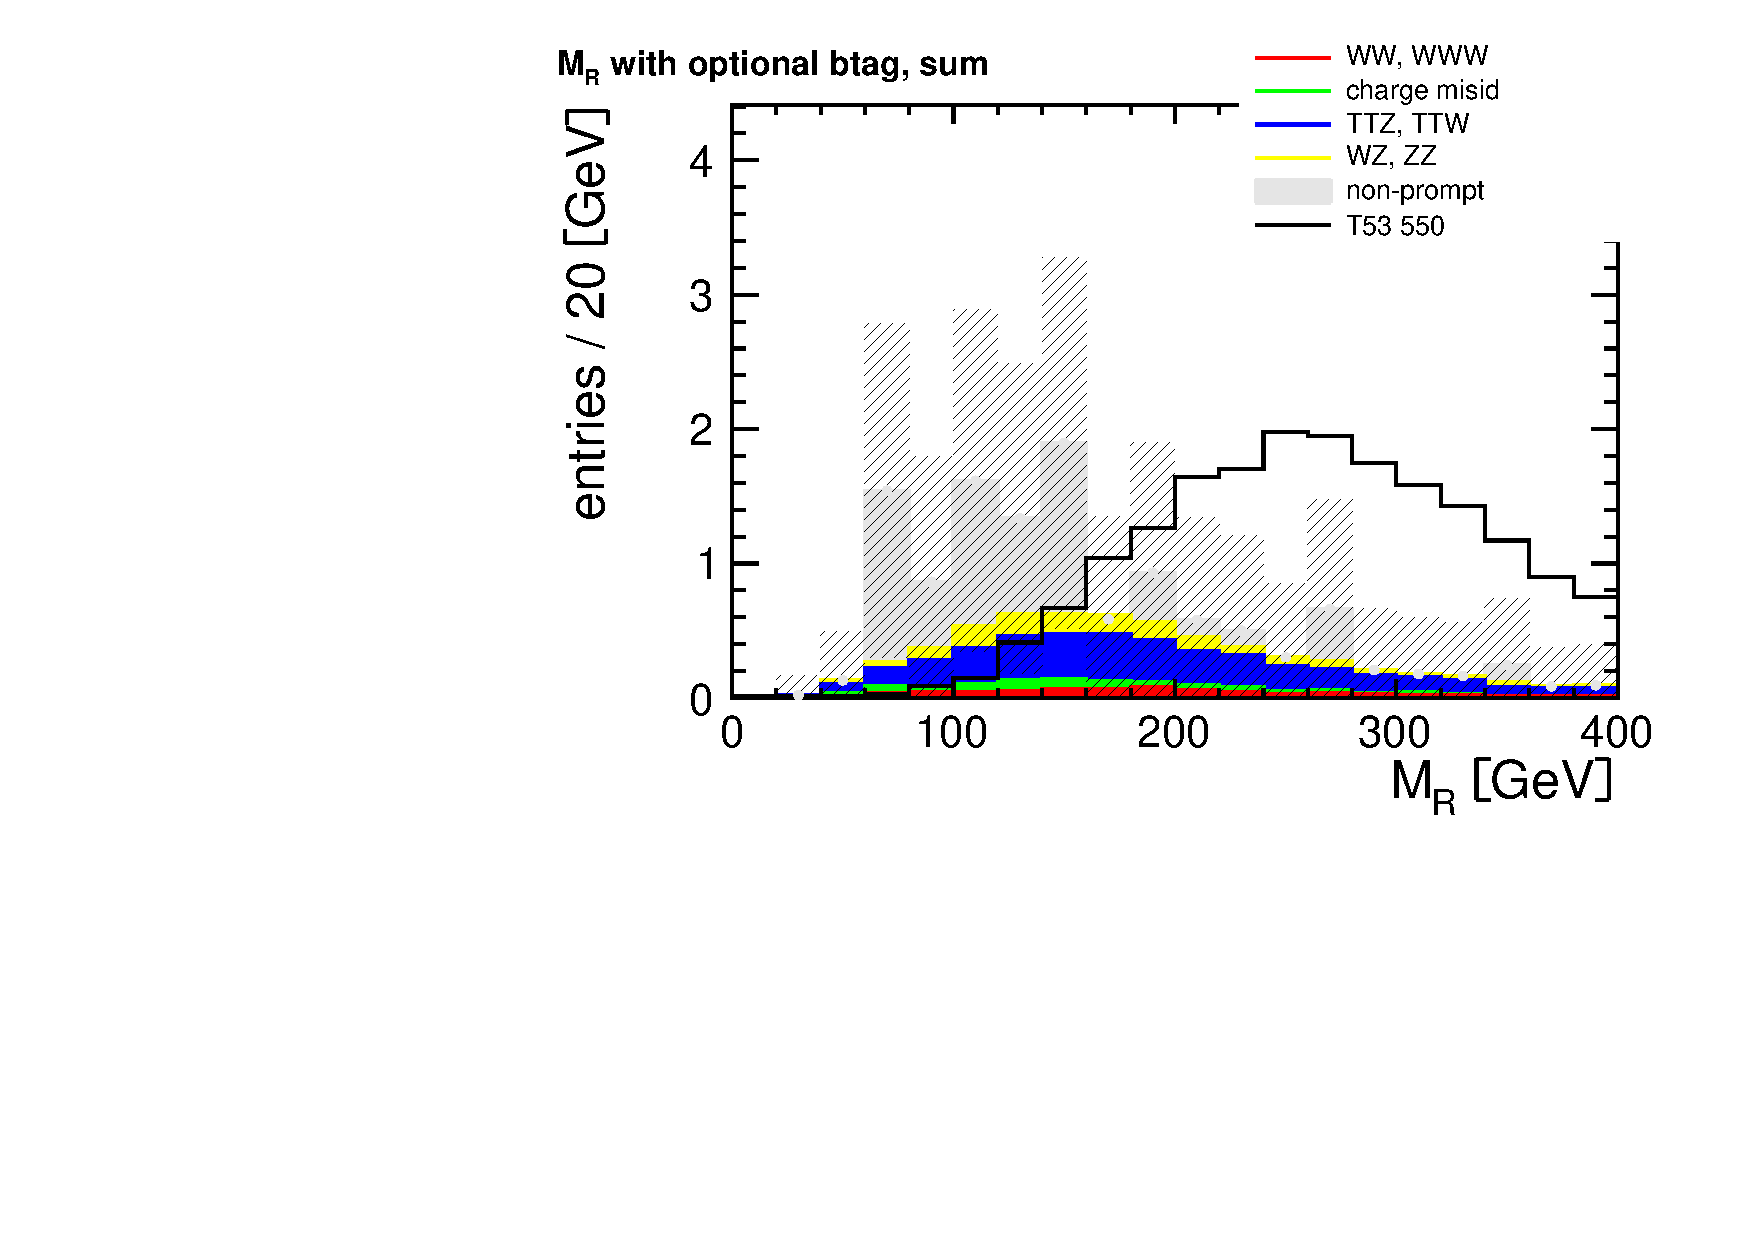
\includegraphics[width=.8\textwidth]{images/pdf/4jets_AND_r02_AND_had_mass350/mr_optional_btag_sum_0}
    \caption{Distribution of the $M_R$ variable for events in the three decay
        channels, with the final
    selection applied without the selection on $M_R$.}
    \label{fig:nomr}
\end{figure}

\begin{figure}[htb]
    \centering
    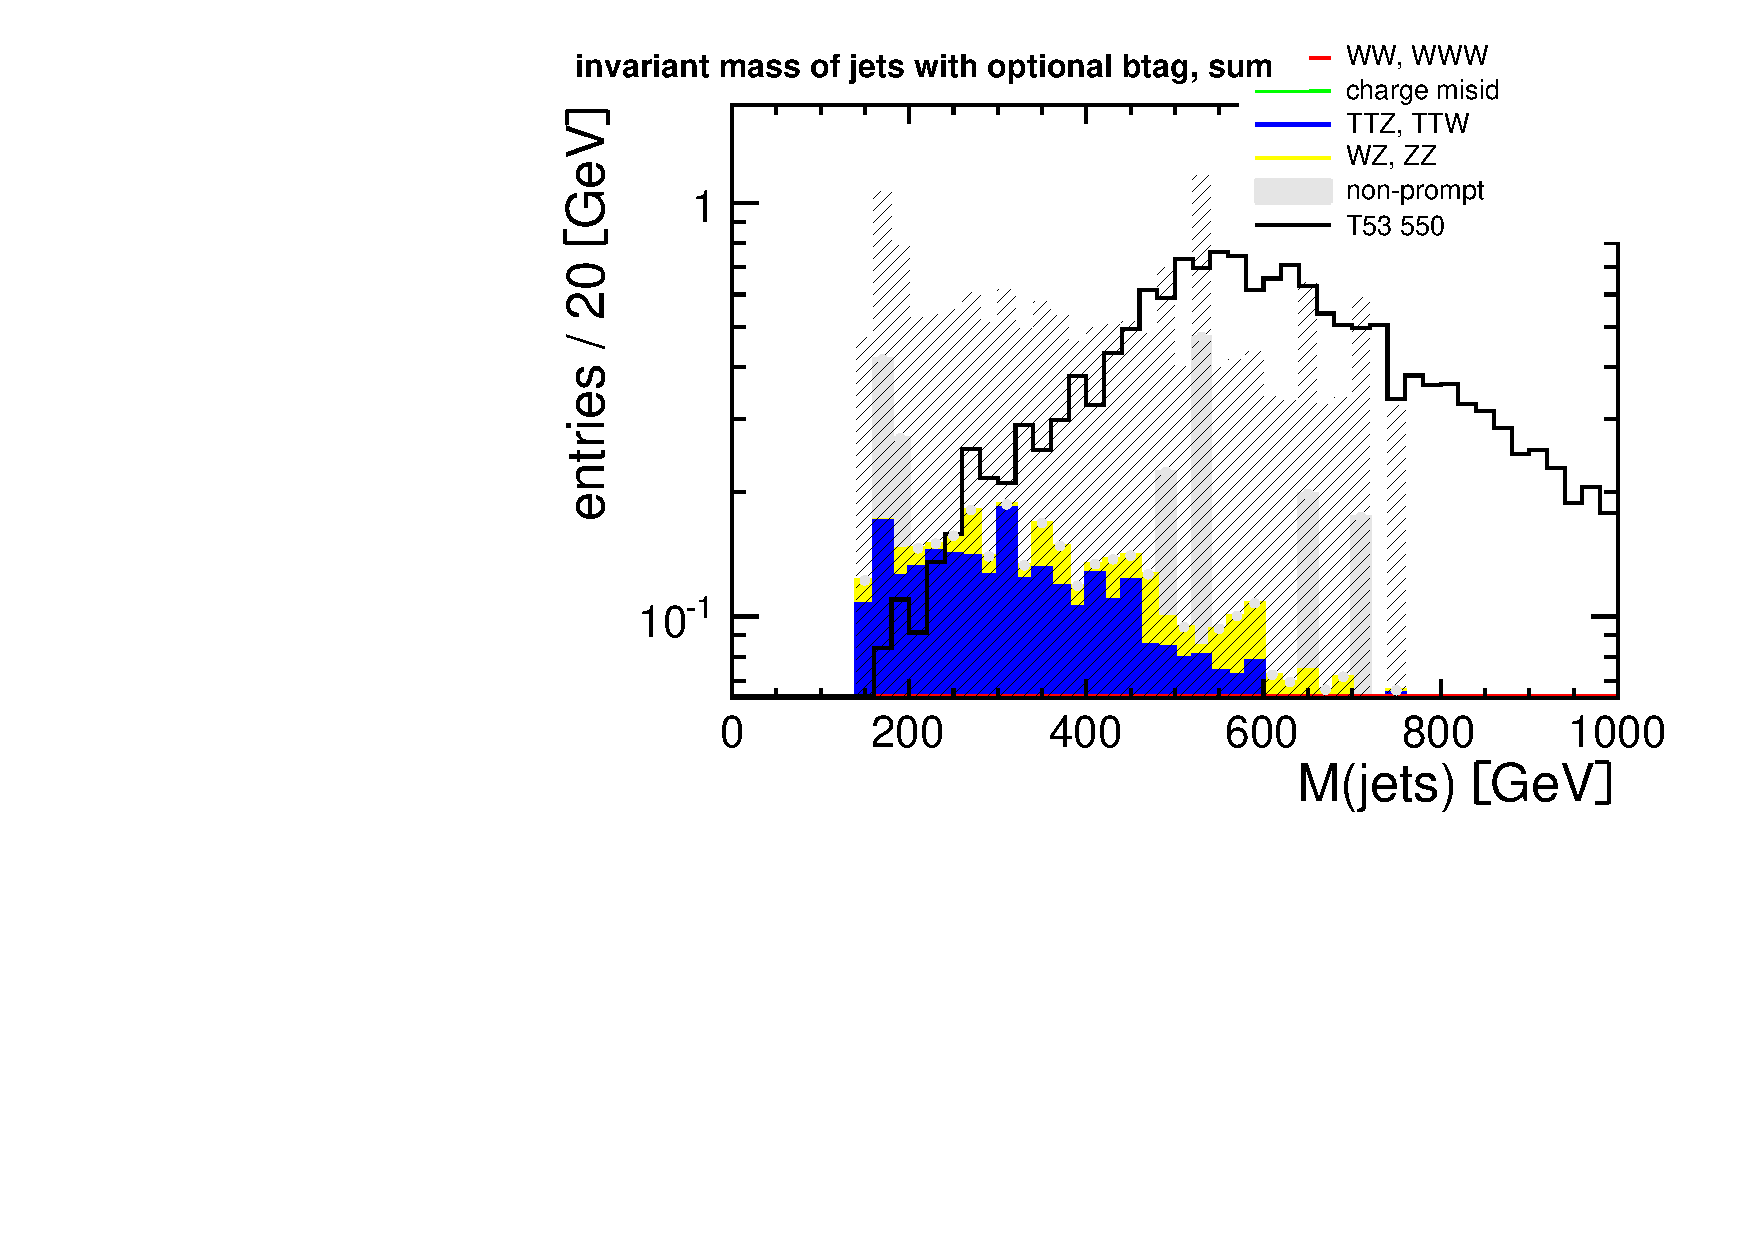
\includegraphics[width=.8\textwidth]{images/pdf/4jets_AND_mr200_AND_r02/had_mass_optional_btag_sum_0}
    \caption{Distribution of the invariant mass of the jets for events in the three decay
        channels, with the final
        selection applied without the selection on $M(\text{jets})$.}
    \label{fig:nohadmass}
\end{figure}
